\documentclass[12pt, a4paper]{article}
\usepackage[english]{babel}             % Inglés para los nombres
\usepackage[utf8]{inputenc}             % Codificación de entrada
\usepackage[T1]{fontenc}                % Codificación de fuente (escribir castellano)
\usepackage{lmodern}                    % Fuente (la default no es compatible con castellano)
\usepackage{csquotes}                   % Para comillas y otras anotaciones del castellano
\usepackage{fancyhdr}                   % Encabezado y Pie de pagina
\usepackage{tocloft}                    % Puntos en los índices

\usepackage{url}                        % 
\usepackage{hyperref}                   % Links y referencias dentro del texto
\usepackage{nameref}                    % Para poder referenciar por nombre
\usepackage{acronym}                    % Para incluir las listas de abreviaturas
\usepackage{multicol}                   % Permite crear espacios con columnas verticales
\usepackage{booktabs} % Para mejores líneas horizontales en tablas
\usepackage{parskip}                    % Eliminar sangrado y añadir espacio entre párrafos
\usepackage{titlesec}                   % Crear subsubsub secciones
\usepackage{amsmath}                    % Funciones para ecuaciones
\usepackage{blkarray}                   % Matrices con anotaciones
\usepackage{algorithm}                  % Algoritmos con formalismos
\usepackage{algpseudocode}              % También para algoritmos
\usepackage{listings}                   % Para insertar codigo

\usepackage{array}                      % Para personalizar columnas de tabla
\usepackage{tabularx}                   % Para tablas de ancho variable

\usepackage{graphicx}                   % Para incluir imágenes
\usepackage{subcaption}                 % Subfiguras
\usepackage[table]{xcolor}              % Definir y utilizar colores
\usepackage{tikz}                       % Dibujar formas, figuras, rectas, intersecciones...
\usepackage[absolute,overlay]{textpos}  % Posición absoluta para textos
\usepackage{geometry}                   % Para controlar los márgenes

\usepackage{float}
\usepackage{soul}                       % Para highligths \hl
\usepackage{lipsum} 

\usepackage[backend=biber, sorting=none]{biblatex} % Referencias (bibliografía / webgrafía)
\selectlanguage{english}                % Seleccionar inglés
\bibliography{references}               % Incluir el archivo de referencias

\setlength{\emergencystretch}{3em}

% Definición de nombres
%\printbibliography[title={Bibliografía}]
\renewcommand{\cftsecleader}{\cftdotfill{\cftdotsep}} 
\newcommand{\student}{García Justel, Alan}
\newcommand{\director}{ Barrena Orueechebarria, Nagore; Elordi Hidalgo, Unai}
\newcommand{\codirector}{Sánchez Juanola, Martí}
\newcommand{\master}{ COMPUTATIONAL ENGINEERING AND INTELLIGENT SYSTEMS}
\newcommand{\titulo}{BEV2SEG\_2: DRIVEABLE AREA SEGMENTATION FOR PREANNOTATION TASKS}
\newcommand{\portada}{images/shared/lomoya.png}
\newcommand{\curso}{2024-2025}

% Definición de Macros
\newcommand*{\fullref}[1]{\hyperref[{#1}]{\autoref*{#1} \nameref*{#1}}} % One single link

\newcommand{\aclink}[1]{% Crear links a acronimos
  \ifcsdef{ac@#1}{%
    \ifcsdef{mark@#1}{%
      \hyperlink{acro:#1}{\acs{#1}}%
    }{%
      \hyperlink{acro:#1}{\ac{#1}}%
      \expandafter\gdef\csname mark@#1\endcsname{}%
    }%
  }{%
    \ac{#1}%
    \expandafter\gdef\csname mark@#1\endcsname{}%
  }%
}

% Notas en Figuras
\newcommand\fnote[1]{\captionsetup{width=0.8\linewidth, font=footnotesize}\caption*{#1}}

% Estilos de listings
% Configuración del estilo para resaltar el código de ROS
\lstdefinestyle{ros}{
    backgroundcolor=\color{white}, % Cambiar el color de fondo
    basicstyle=\small\ttfamily, % Texto más pequeño
    breaklines=true,
    language=C,
    morekeywords={int32, float64},
    keywordstyle=\color{blue},
    commentstyle=\color{green!40!black},
    stringstyle=\color{red},
    breakatwhitespace=false,         
    breaklines=true,                 
    captionpos=b,                    
    keepspaces=true,                 
    numbers=left,                    
    numbersep=5pt,                  
    showspaces=false,                
    showstringspaces=false,
    showtabs=false,                  
    tabsize=2
}

% Crear subsubsub secciones
\titleclass{\subsubsubsection}{straight}[\subsection]
\newcounter{subsubsubsection}[subsubsection]
\renewcommand\thesubsubsubsection{\thesubsubsection.\arabic{subsubsubsection}}
\renewcommand\theparagraph{\thesubsubsubsection.\arabic{paragraph}} % optional; useful if paragraphs are to be numbered

\titleformat{\subsubsubsection}
  {\normalfont\normalsize\bfseries}{\thesubsubsubsection}{1em}{}
\titlespacing*{\subsubsubsection}
{0pt}{3.25ex plus 1ex minus .2ex}{1.5ex plus .2ex}
\makeatletter
\renewcommand\paragraph{\@startsection{paragraph}{5}{\z@}%
  {3.25ex \@plus1ex \@minus.2ex}%
  {-1em}%
  {\normalfont\normalsize\bfseries}}
\renewcommand\subparagraph{\@startsection{subparagraph}{6}{\parindent}%
  {3.25ex \@plus1ex \@minus .2ex}%
  {-1em}%
  {\normalfont\normalsize\bfseries}}
\def\toclevel@subsubsubsection{4}
\def\toclevel@paragraph{5}
\def\toclevel@paragraph{6}
\def\l@subsubsubsection{\@dottedtocline{4}{7em}{4em}}
\def\l@paragraph{\@dottedtocline{5}{10em}{5em}}
\def\l@subparagraph{\@dottedtocline{6}{14em}{6em}}
\makeatother
\setcounter{secnumdepth}{4}
\setcounter{tocdepth}{4}



% Encabezado y Pie de pagina
\pagestyle{fancy}                       % Estilo de las páginas
\fancyhf{}
\fancyhead[L]{Master's Thesis}
\fancyhead[R]{\leftmark}
\fancyfoot[L]{UPV/EHU}
\fancyfoot[R]{\thepage}
\renewcommand{\footrulewidth}{0.4pt} % Línea horizontal en el pie de página
\setlength{\headheight}{15.5pt}

% Definición de colores
\definecolor{ehu_blue}{HTML}{376092}
\definecolor{link_color}{HTML}{36AEB4}
\definecolor{reference_color}{HTML}{0F3133}
\definecolor{cite_color}{HTML}{ff7f42}
\definecolor{table_gray}{HTML}{C0C0C0}
\definecolor{table_red}{HTML}{fb4952}

% Palette colors
\definecolor{palette_red_1}{HTML}{F44336}
\definecolor{palette_red_2}{HTML}{EF5350}
\definecolor{palette_red_3}{HTML}{F1464E}
\definecolor{palette_yellow_1}{HTML}{FF9800}
\definecolor{palette_green_1}{HTML}{4CAF50}
\definecolor{palette_green_2}{HTML}{86BB48}
\definecolor{palette_green_3}{HTML}{39C39E}
\definecolor{palette_blue_1}{HTML}{0277BD}
\definecolor{palette_blue_2}{HTML}{0097A7}
\definecolor{palette_blue_3}{HTML}{2AB0D2}

% Incluye todas las entradas del archivo .bib en la bibliografía
\nocite{*}

% Configuración de hyperref para diferentes tipos de enlaces
\hypersetup{
    colorlinks=true,
    linkcolor=reference_color,
    citecolor=cite_color,
    filecolor=link_color,
    urlcolor=link_color,
}

% #########################################################################
% #                                  TFM                                  #
% #########################################################################
\begin{document}
\newgeometry{bottom=2cm}

\begin{titlepage}
    % Logo de la universidad
    \begin{textblock*}{\textwidth}(10cm,0cm)
        
\includegraphics[width=7.5cm, height=3cm]{images/shared/Logo_EHU.jpg}
    \end{textblock*}
    
    % Franja azul
    \begin{tikzpicture}[remember picture, overlay]
        \fill[ehu_blue] (current page.north west) ++ (0,-3.01cm) rectangle (\paperwidth,-3cm);
    \end{tikzpicture}
    
    \begin{textblock*}{\paperwidth}(\dimexpr\parindent+\oddsidemargin+3em\relax,3.5cm)
        \begin{minipage}{\dimexpr\linewidth-7.5cm\relax}
            \color{white}
            \noindent\rule{\linewidth}{0cm}
            \textsf{ {\large MÁSTER EN \master}}
            \newline
            \newline \newline
            \textsf{\textbf{ {\Huge TRABAJO FIN DE MÁSTER }}}
        \end{minipage}
    \end{textblock*}
    
    % Título del trabajo
    \vspace*{3.5cm}
    \begin{minipage}{\linewidth}
        \setlength{\baselineskip}{1.7\baselineskip}
        \centering
        \textsf{ \textbf{ {\LARGE \titulo }}}
    \end{minipage}

    % Foto de portada
    \vspace*{0.5cm}
    \begin{figure}[H]
        \centering
        \includegraphics[width=10cm, height=8cm]{\portada}
    \end{figure}

    % ODS
    \vspace*{1cm}
    % \begin{figure}[h]
    % \centering
    %     \begin{subfigure}[b]{0.135\textwidth}
    %         \includegraphics[width=2cm, height=2cm]{images/iconos_ods/03.png}
    %     \end{subfigure}
    %     \begin{subfigure}[b]{0.135\textwidth}
    %         \includegraphics[width=2cm, height=2cm]{images/iconos_ods/04.png}
    %     \end{subfigure}
    %     \begin{subfigure}[b]{0.135\textwidth}
    %         \includegraphics[width=2cm, height=2cm]{images/iconos_ods/05.png}
    %     \end{subfigure}
    %     \begin{subfigure}[b]{0.135\textwidth}
    %         \includegraphics[width=2cm, height=2cm]{images/iconos_ods/07.png}
    %     \end{subfigure}
    %     \begin{subfigure}[b]{0.135\textwidth}
    %         \includegraphics[width=2cm, height=2cm]{images/iconos_ods/08.png}
    %     \end{subfigure}
    %     \begin{subfigure}[b]{0.135\textwidth}
    %         \includegraphics[width=2cm, height=2cm]{images/iconos_ods/09.png}
    %     \end{subfigure}
    %     \begin{subfigure}[b]{0.135\textwidth}
    %         \includegraphics[width=2cm, height=2cm]{images/iconos_ods/12.png}
    %     \end{subfigure}
    % 
    %     \label{fig:ods-iconos}
    % \end{figure}
    
    % Estudiante
    \vspace{0.2cm}
    \noindent {\footnotesize \textbf{Estudiante:} \estudiante}
    \newline
    \noindent\makebox[\linewidth]{\rule{\textwidth}{0.4pt}} % Línea horizontal

    % Director
    \nopagebreak
    \vspace{0.3cm}
    \nopagebreak
    \noindent {\footnotesize \textbf{Director/Directora:} \director }

    % Espacio para firmas
    \vspace{0.5cm} % Espacio entre texto "Director/Directora" y espacio para firmas
    \noindent 
    \makebox[0.4\linewidth]{\hrulefill}
    \hspace{0.2\linewidth}
    \makebox[0.4\linewidth]{\hrulefill}

    % Curso y Fecha
    \vspace{0.1cm}    
    \noindent {\footnotesize \textbf{Curso: } \curso \hfill \textbf{Fecha:} \today }
\end{titlepage}

\restoregeometry
\setcounter{figure}{0} % Incluimos el título

% \newpage % BORRAR EN LA VERSIÓN FINAL
% \input{notas}

\newpage
\markboth{Abstract}{Abstract}
\begin{itshape}
    \textbf{Abstract:} \\

Automated Driving Systems (ADS) critically depend on robust perception systems capable of generating reliable environmental representations. Bird's-Eye View (BEV) maps are fundamental for this, as they offer an unified, top-down 2D representation of the vehicle's immediate surroundings. While traditional methods for generating BEV semantic segmentation maps from camera data rely on a previous semantic segmentation of the perspective camera-image followed by Inverse Perspective Mapping (IPM), this approach is limited by assumptions of flat ground and distortion for taller objects. While recent data-driven techniques address these limitations, the specific impact of directly training semantic segmentation models on BEV images to see if it better segments planar elements remains underexplored.

This master's thesis investigates whether training a semantic segmentation model directly on BEV images outperforms the traditional image-space segmentation followed by IPM reprojection, particularly for planar elements as they get a metric representation in the BEV domain. To address this, a novel BEV2Seg\_2 framework is developed, enabling a direct comparison between these two strategies. Contrary to the initial hypothesis, experiments consistently demonstrated that the traditional Segmenting-Then-IPM strategy yielded superior segmentation performance for both obstacles and planar elements. Additionally, this work found that modifying camera extrinsic parameters for BEV data augmentation was more effective than traditional geometric augmentations, significantly reducing model overfitting.

Beyond this comparative analysis, this work also explores a practical application by developing an automated pre-annotation pipeline to generate BEV masks for occupancy, occlusion, and driveable areas.  While this pipeline has some limitations, especially with partially occluded objects, it produces reliable enough masks for valuable downstream tasks in autonomous driving, such as scene reconstruction and path planning. 

In summary, this thesis provides a robust experimental foundation demonstrating that traditional Segmenting-Then-IPM offers superior performance in BEV semantic segmentation, and presents a functional pre-annotation system that advances autonomous driving perception.

    \textbf{Keywords: Automated Driving Systems (ADS), BEV Semantic Segmentation, Automated Annotation, Computer Vision, Occupancy Mapping, Occlusion Estimation}
\end{itshape}
\newpage
 

% Índices
\tableofcontents\thispagestyle{empty}\newpage
\listoffigures\thispagestyle{empty}\newpage
\listoftables\thispagestyle{empty}\newpage

% Abreviaturas
\section*{Acronyms}
\markboth{Acronyms}{Acronyms}
\addcontentsline{toc}{section}{Acronyms}
%\begin{multicols}{2} % Si se quieren en dos columnas verticales
\begin{acronym}[ADAS]  % El acrónimo más largo
    \acro{TFM}{Trabajo Fin de Máster}
    \acro{ADS}{Automated Driving Systems}
    \acro{ADAS}{Advanced Driving Assistance Systems}
    \acro{SAE}{Society of Automotive Engineers}
    \acro{V2I}{Vehicle-to-Infrastructure}
    \acro{V2X}{Vehicle-to-Everything}
    \acro{BEV}{bird's-eye-view}
    \acro{LiDAR}{Light Detection and Ranging}
    \acro{IPM}{Inverse Perspective Mapping}
    \acro{MLP}{Multilayer perceptron}
    \acro{CNN}{Convolutional Neural Network}
    \acro{FCN}{Fully Convolutional Network}

\end{acronym}
%\end{multicols}

 % Marcar como visto (No te desglosa el acrónimo)
 % Provoca warnings pero funciona :)
\acused{ADAS}
\acused{LiDAR}
\acused{FCN}
\newpage

\section{Introduction}
\label{Introduction}
% ================================================
% =                INTRODUCTION                  =
% ================================================ 

The development of \aclink{ADS} has been a hot topic in the automotive industry for the last years. One of the fundamental aspects of an \aclink{ADS} is its perception system, as it is responsible for performing the obstacle detection and to provide a good environment representation for other systems, among others. This perception system can be divided into two main tasks: 3D object detection and local \aclink{BEV} map generation. 

3D object detection is usually based on pointclouds obtained from \aclink{LiDAR} sensors, but as this sensors are costly a lot of research has been made in the field of camera 3D object detection. This approach has been gaining a lot of popularity carried by the improvemnts of the computer vision techniques with deep learning.

\aclink{BEV} segmentation aims to create a semantic representation of a vehicle's surroundings. This is a key component of an \aclink{ADS} perception system as \aclink{BEV} segmentation provides rich semantic information, precise localization, and absolute scales. This makes it useful for various tasks, including map reconstruction, prediction of agent intentions, and vehicle path planning.

To obtain \aclink{BEV} semantic segmentation from cameras, traditional methods first generate semantic masks in image space and then transform them into \aclink{BEV} space using \aclink{IPM}. Although simple, it requires accurate camera parameters and assumes a perfectly flat ground surface, which limits its effectiveness. Moreover, while planar or low-height objects such as road curbs, lane markings, and the drivable area retain a meaningful metric representation in \aclink{BEV} space, objects with height appear distorted after the transformation.

With the objective of addressing this limitations, recent methods leverage data-driven techniques for \aclink{BEV} representation. \cite{view_parsing_network} \cite{lift_splat_shoot} \cite{m2bev}. However, to the best of our knowledge, no previous work has explored training a standard semantic segmentation model directly on \aclink{BEV} images to measure the difference between the inference of planar elements.

This master's thesis seeks to answer the question: \textit{Does a model directly trained on semantic BEV images outperforms a typical segmentation model for plannar elements?}. Additionally, this work explores a technical application of \aclink{BEV} semantic segmentation for annotating vehicular scenes with occupancy, occlusion, and drivable area masks, contributing to the field of monocular 3D object detection given 2D semantic masks.


\newpage

\section{State of the art}
\label{sota}
% ================================================
% =              STATE OF THE ART                =
% ================================================ 
Actualmente, la industria de la automoción está impulsando el desarrollo de los \aclink{ADS} con la promesa de reducir los accidentes en carretera y minimizar los costes tanto humanos como económicos que estos suponen \cite{survey_AutomatedDriving1}. Sin embargo, a pesar de que la conducción automatizada haya incrementado recientemente la atención de la industria por el auge del DeepLearning y la visión por ordenador, lo cierto es que lleva presente más de 20 años.

Algunas de las primeras competiciones de conducción automatizada, como los DARPA Challenges en 2003 y 2005 o el Grand DARPA Urban challenge de 2007, impulsaron enormemente el desarrollo de los \aclink{ADS}, atrayendo la atención tanto de empresas tecnológicas como del sector automotriz \cite{survey_AutomatedDriving2}. Este avance ha sido acompañado por la definición de buenas prácticas y procesos de estandarización para garantizar la seguridad y fiabilidad de los \aclink{ADS}. En este contexto, la \aclink{SAE} ha establecido una escala progresiva de automatización, desde el nivel 0 (sin automatización) hasta el nivel 5 (automatización total), definiendo el grado de intervención del conductor en cada etapa \cite{AD_Technical_Standards}. 

Hoy en día, la mayoría de los vehículos incorporan sistemas avanzados de asistencia a la conducción \aclink{ADAS}, que operan en los niveles \aclink{SAE} 2 y 3. No obstante, ya existen \aclink{ADS} de nivel 4, como los desarrollados por Waymo y Cruise para robotaxis, o los autobuses autónomos desplegados en algunas ciudades, cuyos sistemas están diseñados para gestionar el fallback de manera autónoma, sin necesidad de intervención humana \cite{fallback_strategy}.

Este desarrollo ha llevado a la creación de distintas estrategias y arquitecturas para los \aclink{ADS}. En los últimos años, ha habido grandes avances en soluciones \mbox{End-to-End}, que combinan técnicas de aprendizaje profundo y aprendizaje por refuerzo para obtener las acciones de control del vehículo partiendo diréctamente de los datos de los sensores \cite{end_to_end_driving}. Sin embargo, la mayoría de los enfoques optan por soluciones modulares más tradicionales, que dividen el problema de la conducción automatizada en \mbox{sub-tareas} específicas, integrando soluciones de campos como la robótica, visión por ordenador, deep learning y control automático.

En el contexto de las arquitecturas modulares, la adopción de buenas prácticas ha facilitado la categorización de estas \mbox{sub-tareas} en tres grupos principales \cite{machines5010006}\cite{functional_architectures}: 
\begin{itemize}
    \item Percepción, que se refiere a la capacidad del sistema autónomo para recolectar información del entorno y extraer conocimiento relevante, como la ubicación de obstáculos, señales de tráfico y la localización del vehículo.
    \item Planificación del comportamiento, que consiste en tomar decisiones para alcanzar los objetivos del vehículo, como llegar de un punto a otro evitando obstáculos y optimizando la trayectoria.
    \item Ejecución de movimientos, que se refiere a la capacidad del vehículo para ejecutar las acciones planificadas por el sistema, controlando la dirección, velocidad y maniobras necesarias.
\end{itemize}
Además, estas \mbox{sub-tareas} interactúan entre sí, con el hardware del vehículo y con sistemas de comunicación como \aclink{V2I} o \aclink{V2X} en el caso de los vehículos conectados.

\begin{figure}[H]
    \centering
    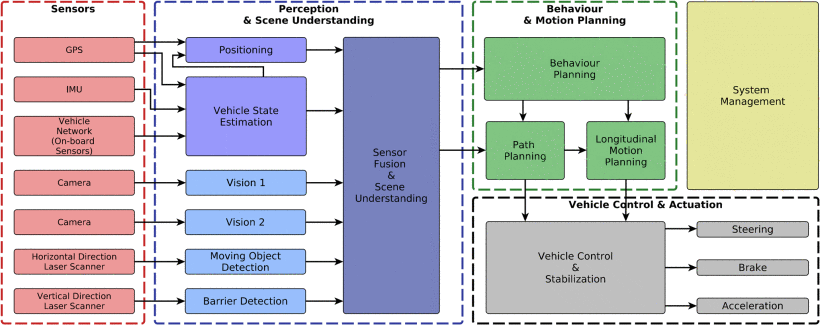
\includegraphics[width=\linewidth]{images/sota/ADS_information_flow.png}
    \label{sota_ads_information_flow}
    \caption{Arquitectura modular de un ADS. TEMPORAL!!!}
\end{figure}

En este tipo de arquitecturas, un error en una \mbox{sub-tarea} puede propagarse y afectar el desempeño de otras, comprometiendo así el funcionamiento del sistema. Esto es especialmente crítico en el módulo de percepción, ya que la calidad de la información obtenida impacta directamente en tareas posteriores como la localización, el mapeo y la planificación. Por ello, garantizar sistemas de percepción robustos es fundamental para el rendimiento y la seguridad de los \aclink{ADS}.

Dos de las tareas principales de los sistemas de percepción en los \aclink{ADS} son la detección 3D de objetos y la segmentación en \aclink{BEV}. La detección 3D de objetos es una de las tareas más relevantes y comúnmente se basa en nubes de puntos obtenidas mediante sensores LiDAR. En ausencia de LiDAR, una alternativa es la detección 3D multi-cámara, que busca predecir cajas delimitadoras 3D en un sistema de coordenadas \aclink{BEV} utilizando únicamente imágenes monoculares. Por otro lado, la segmentación en \aclink{BEV} tiene como objetivo realizar una segmentación semántica del entorno, identificando áreas transitables y delimitaciones de carril en el marco de referencia del vehículo. A diferencia de la detección de objetos, la segmentación en \aclink{BEV} permite una predicción densa de clases estáticas del entorno, lo que resulta clave para la construcción de mapas locales, estimación del comportamiento de agentes y downstream tasks como la planificación del comportamiento del \aclink{ADS}. \hl{Añadir referencias.}

% Parrafo conector que no se me ocurre nada
Este \aclink{TFM} se desarrolla en el contexto de la segmentación semántica en \aclink{BEV}\dots \hl{COMPLETAR.}


\subsection{Semantic segmentation}
\lipsum[2-4] % TODO

\subsection{BEV semantic segmentation}

% TODO: Esto es una piedra de ChatGPT y hay varios errores. Reescribir todo.
%       Alguna imagen no estaría de más.
%

Traditional methods (3D\_Traffic\_Scene\_Understanding) estimate local BEV maps using multi-camera input under the flat-ground assumption, applying Inverse Perspective Mapping (IPM). However, these methods require accurate camera parameters, which has led to research focusing on camera parameter estimation for BEV transformation (BEV\_Params\_Estimation1, BEV\_Params\_Estimation2).

Cam2BEV applies IPM to transform multi-camera input images into BEV space and refines the representation using homographies fed into the model. To handle occlusions, Cam2BEV introduces an additional semantic class that explicitly marks occluded areas from all vehicle-mounted cameras, improving the final BEV estimation.

HDMapNet generates high-definition semantic maps from multi-camera input by employing a feature projection module that transforms image features into BEV space. It models the 3D environment implicitly using an MLP and explicitly incorporates camera extrinsic parameters to project image-space features correctly into BEV. The model first extracts image features with a shared MLP backbone, transforms them into the camera coordinate system, and then projects them into BEV using camera extrinsics.

PYVA introduces a cross-view transformer that projects features from the front-view domain to the BEV domain. While similar to HDMapNet, PYVA differs in that it does not rely on camera parameters in the second transformation stage. Instead, it employs a GAN-based framework to manage occlusions, making it applicable for monocular settings but less suitable for multi-camera fusion.

Other approaches propose different architectures for BEV semantic segmentation. VPN introduces a two-layer MLP for multi-camera feature fusion, followed by a decoder for semantic segmentation in indoor environments. LSS presents a unified framework that lifts 2D images into 3D space by learning an implicit depth distribution, making it effective for end-to-end motion planning. M²BEV transforms 2D image features into 3D voxels along projection rays to generate an efficient BEV representation that supports tasks such as semantic segmentation and 3D object detection. BEVFormer, on the other hand, employs a transformer-based approach that aggregates spatial-temporal features from multi-view cameras and historical BEV frames, enhancing occlusion reasoning.

MonoLayout tackles occlusion estimation by employing a standard encoder-decoder framework combined with adversarial training, enabling it to predict amodal layouts of the driving scene. BEVFormer similarly enhances occlusion reasoning by leveraging attention mechanisms to fuse multi-view spatial-temporal features from historical BEV maps.

Several methods integrate multiple sensor modalities to improve BEV representations. FishingNet extends VPN by incorporating data from additional sensors, while HDMapNet also supports LiDAR fusion, allowing for a more detailed understanding of the driving environment.

To the best of our knowledge, Cam2BEV is the closest approach to this thesis. However, our work differs in several key aspects. Instead of applying semantic segmentation after transforming images into BEV space, we study whether training a segmentation model directly on BEV images improves the representation of planar elements compared to the traditional segmentation-first-then-IPM approach. Furthermore, we treat occupancy and occlusion mask generation as a post-processing step applied to BEV semantic segmentation. This is integrated into a pre-annotation pipeline for vehicle scenes, contributing to advancements in monocular 3D object detection.


\newpage

\section{Metodology}
\label{metodologia}

% En esta sección se detallan los experimentos realizados para abordar las cuestiones propuestas en la sección \ref{Introduction}. En primer lugar, se introducen los detalles del diseño de la experimentación: la selección del modelo de segmentación, dataset elegido, procesos de entrenamiento y validación, etc. Después, se detalla el pipeline implementado para realizar la anotación semiautomática de las máscaras de ocupación, oclusión y área conducible. Finalmente, se aborda la metodología seguida para evaluar tanto la generación de las máscaras semánticas en \aclink{BEV}, como las detecciones 3D a partir de imágenes monoculares para la evaluación final del pipeline de anotación semiautomática.

This section details the experiments and implementations made to address the problems described in section \ref{Introduction}. On the first hand, the experimental design is introduced, tackling the model and dataset selection, how data augmentations are performed and the training and validation processes. Afterward, the implementation of the occupancy and occlusion masks preannotation pipeline is presented. Finally, the evaluation strategy of the pipeline is discussed to measure the quality of the resulting semantic masks and the monocular 3D detections for estimating the object's dimensions.

% Este proyecto puede dividirse en 3 bloques principales: experimentación con la segmentación semántica en BEV, diseño e implementación de un sistema de anotación semiautomático de máscaras de área conducible y un tercer bloque de experimentación para evaluar el rendimiento del sistema implementado.

Thus, this project can be divided into three main blocks: \aclink{BEV} semantic segmentation experimentation, design and implementation of the preannotation pipeline and a thrid block of how the system is evaluated.

\subsection{Segmentation experiment design: BEV2Seg\_2}
\label{bev2seg_2}

To address the hypotesis that "A semantic segmentation model trained with BEV images better segments planar elements" the process represented in Figure \ref{fig:beg2seg_2_flow} has been designed. It follows two main approaches: first, performing image segmentation on regular RGB images and then reprojecting them to \aclink{BEV}; second, applying \aclink{IPM} to the original images and then segmenting them with the model.

\begin{figure}[h!]
    \centering
    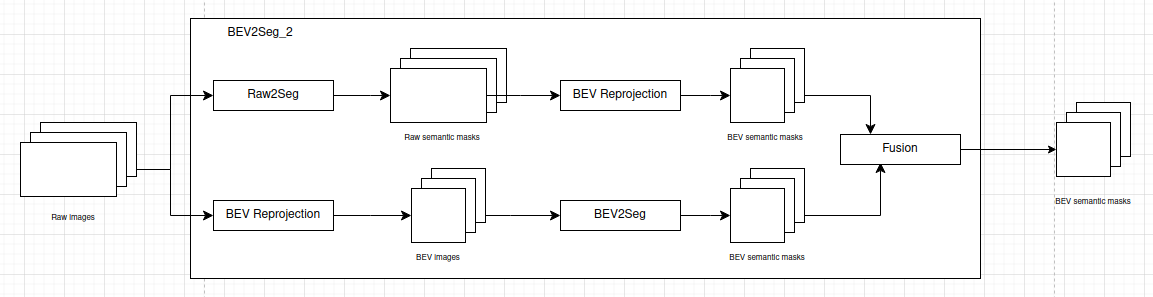
\includegraphics[width=\linewidth]{./images/metodology/bev2seg_2_flow.png}
    \caption{bev2seg\_2 diagram flow.}
    \label{fig:beg2seg_2_flow}
\end{figure}

Considering this flowchart, three main questions arises: (1) which segmentation model to use, (2) which dataset to train the models with, and (3) how to compare the train models and select the optimal output of the pipeline. 

\subsubsection{Segformer}
There are multiple techniques and strategies for tackling semantic segmentation in both regular and \aclink{BEV} images \ref{sota}.  

Several models could be chosen to address the proposed hypothesis. The current state of the art includes both \aclink{CNN} and \aclink{ViT}-based models that achieve competitive results. As shown in Figure \ref{tab:model_comparison}, there is no significant difference in accuracy and inference speed among the top-performing models. Moreover, many of these models have already been applied in the context of \aclink{ADS}. In this work, Segformer \cite{segformer} has been selected as the semantic segmentation model due to its balance between performance and efficiency. Additionally, it is integrated into the Huggingface \cite{huggingface} ecosystem, which provides an optimized, parallelized implementation, facilitating distributed training.  

\begin{table}[h]
    \centering
    \resizebox{\linewidth}{!}{%
    \begin{tabular}{l l c c c}
        \toprule
        \textbf{Model Name} & \textbf{Encoder} & \textbf{Params (M)} $\downarrow$ & \textbf{FPS} $\uparrow$ & \textbf{Cityscapes test mIoU ($\%$)} $\uparrow$ \\
        \midrule
        DDRNet-39       & -             & 32.3      & -         & 80.4 \\
        PIDNet-L        & -             & 36.9      & -         & 80.6 \\      
        DeeplabV3+      & ResNet-101    & 62.7      & 1.2       & 80.9 \\
        SETR            & ViT-Large     & 318.3     & 0.5       & 82.2 \\
        Segformer       & MiT-B4        & 64.1      & 3.0       & 83.8 \\
        \bottomrule
    \end{tabular}%
    }
    \caption{Comparison of different models. Results are obtained from \cite{DDRNet} \cite{PIDNet} \cite{segformer}.  }
    \label{tab:model_comparison}
\end{table}


The Segformer model consists on an hierarchical Transformer  encoder, which extract coarse and fine features, and a lightweight \aclink{MLP} decoder to directly fuse these multiscale features and predict the segmentation mask (Figure \ref{fig:segformer_architecture}). Segformer comes with a series of Mix Transformer encoders (MiT) that share the same architecture but have different sizes: from MiT-B0 as the lightweigtest encoder for realtime inference, to MiT-B5 for best performance.

\begin{figure}[h!]
    \centering
    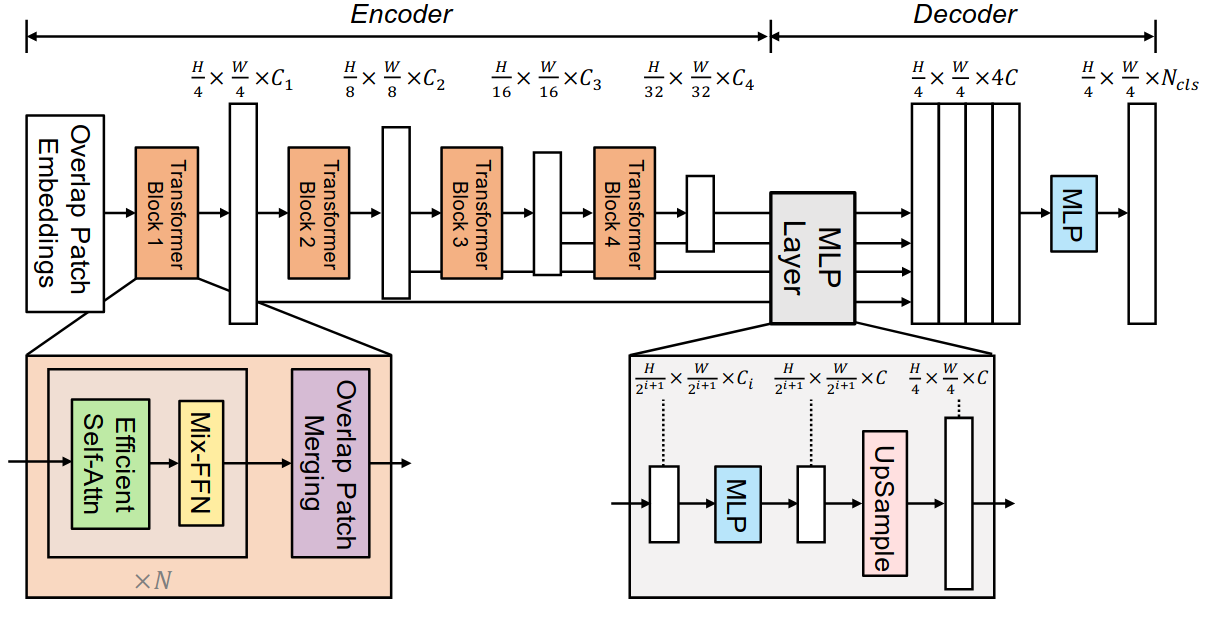
\includegraphics[width=\linewidth]{images/metodology/segformer_architecture.png}
    \caption{Segformer architecture}
    \label{fig:segformer_architecture}
\end{figure}

The training strategy involves using pretrained encoders from ImageNet-1K, attaching an untrained segmentation head decoder, and fine-tuning the entire model for semantic segmentation of vehicular scenes. Since the objective is to train the models directly on \aclink{BEV} images, which differ significantly from standard perspective images, the encoder layers will remain trainable rather than being frozen.


\subsubsection{BEVDataset}
In order to train the model on the segmentation task, a valid dataset must be selected. There are several semantic segmentation datasets for the \aclink{ADS} context such as Cityscapes \cite{Cityscapes}, that defines $30$ semantic classes and provides $5.000$ frames with pixel-level high-quality annotations and $20.000$ weakly annotated images; KITTI \cite{KITTI}, which provices $400$ annotated images with a $0.5$ split for training and validation following the Cityscapes annotation format; ApolloScape \cite{ApolloScape}, that provides $146.997$ frames with corresponding pixel-level annonations and pose information for $25$ labels; or NuImages, a subset of NuScenes \cite{nuscenes}, that contains annotated images on $26$ different labels. For all of them, the ego pose and camera parameters metadata are provided. 

There are other benchmarks \cite{WildDash} \cite{CamVid} but in orther to train the models a rich dataset is needed. Despite Cityscapes and ApolloScape being good options for this task, NuImages has been selected as it is one of the most used datasets for \aclink{ADS} tasks, it provides very accurate ego poses and camera parameters, it has 3D annotations and it has a very good documentation.

NuImages contains around $93.000$ samples with aproximately $80\%$ reserved for the training set and $20\%$ for validation. Additionally, NuImages includes a private test set reserved for benchmark evaluations, whose annotations are not publicly available.

To train the models in the pipeline, a parser has been developed to convert NuImages into a sub-dataset named BEVDataset. This dataset has all front-camera images with NuImages annotations. Since the test annotations in NuImages are private, the validation set has been further splitted to ensure fair comparisons between models from different pipelines.

The conversion process is performed using a custom parser named "OLDatasets", which transforms NuImages samples into the structured ASAM OpenLABEL \footnote{\url{https://www.asam.net/standards/detail/openlabel/}} format, where metadata for each frame is stored. In the case of BEVDataset, images are reprojected into the \aclink{BEV} domain using the \aclink{VCD} library. This library provides tools to handle OpenLABEL annotations and manage both 2D and 3D data efficiently.

The "OLDatasets" parser extracts the camera parameters for each sample and computes a \aclink{LUT} to apply \aclink{IPM} reprojection. Using this data, semantic pixel masks are generated and reprojected along with the original images into the \aclink{BEV} space. Since this reprojection involves image warping, the interpolation method must be carefully chosen:
\begin{itemize}
    \item Linear interpolation is applied to images.
    \item Nearest neighbor interpolation is used for semantic masks to preserve pixel class integrity. 
\end{itemize}

The virtual \aclink{BEV} camera parameters are fixed: the \aclink{BEV} reprojection is generated using a regular grid with a cell spacing of 1 meter, covering a total distance of 30 meters in front of the camera and 1 meter behind it. The resulting images have a resolution of $1024 \times 1024$ pixels.

Finally, BEVDataset contains a total of $16.427$ images, distributed as shown in Figure \ref{fig:bev_dataset}.

\begin{figure}[h!]
    \centering
    \includegraphics[width=\linewidth]{images/metodology/BEVDataset.png}
    \caption{BEVDataset structure and mini set samples}
    \label{fig:bev_dataset}
\end{figure}


\subsubsection{Data augmentations}
Data augmentations in \aclink{BEV} are not an easy task...

\subsubsection{Validation and comparison}
Mean intersection over union (mIoU) or Jaccard index is used as the metric for evaluation and comparison between the two approaches.

\subsection{ Driveable area automatic annotation}
\label{aplication}

\subsubsection{Depth estimation}
\subsubsection{Scene PCD}
\subsubsection{Instance scene PCD}
\subsubsection{Instance BEV mask}

\subsection{Evaluation methodology}
\label{evaluacion}

\subsubsection{3D detections evaluations}
\subsubsection{BEV masks evaluation}
\hl{Groundtruth BEV masks could be generated from annotations}



\newpage

\section{Experiments and results}
\label{experiments_and_results}
% ================================================
% =                 EXPERIMENTS                  = 
% ================================================ 
\hl{Review this.}

This section includes all experiments carried out for evaluating the difference between the two approaches considered in the BEV2Seg\_2 pipeline, experiments to study what is the influence of extrinsic parameters modification as data augmentation technique for semantic segmentation of BEV images and the final evaluation of the proposed annotation pipeline of occupancy, occlusion and driveable areas.

\subsection{[T4] BEV2Seg\_2 experimentation}

Both approaches, segmenting-then-IPM and IPM-then-segmenting, were trained under the same conditions. During fine-tuning for the segmentation task, encoder layers were left unfrozen, allowing the entire model to adapt to the training data. Input images were preprocessed using the \textit{SegformerImageProcessor}, which includes resizing to $512 \times 512$ pixels, rescaling pixel values by a factor of $1/255$, and normalizing with ImageNet mean and standard deviation values~\cite{imagenet}. This preprocessing step ensures the input format is consistent with what the pretrained encoders expect.

Semantic masks were provided during training with the \texttt{reduce\_labels} parameter set to \texttt{False}, as the dataset includes a "background" class. This configuration ensures that all pixel classes, including background, contribute to gradient computation during optimization. All experiments were executed on the hardware setup described in Table~\ref{tab:hardware}. From the six available Segformer encoder variants, three were selected for evaluation: MiT-b0, MiT-b2, and MiT-b4. Due to its larger size, the MiT-b4 model required two gradient accumulation steps to fit within the GPU's memory constraints. Checkpoints were saved based on evaluation loss, a design decision made despite ongoing discussions about whether loss or mean intersection over union is the better metric for model selection. A basic linear learning rate scheduler was applied throughout training and the loss function employed was \texttt{BCEWithLogitsLoss}, which is well-suited for multi-label semantic segmentation tasks, as it combines sigmoid activation and binary cross-entropy in a numerically stable way following the Segformer implementation.

\begin{table}[h]
    \centering
    \begin{tabular}{c l c}
        \toprule
        \textbf{Component} & \textbf{Specifications} & \textbf{Num workers} \\
        \midrule
        CPU         & Intel Xeon Gold 6230 (80) @ 3.900GHz & 8 \\
        GPU         & NVIDIA Tesla V100-SXM2-32GB & 2 \\      
        Memmory     & 772643MiB & - \\
        OS          & Ubuntu 22.04.3 LTS x86\_64 & - \\
        \bottomrule
    \end{tabular}
    \caption{ Hardware used for experiments }
    \label{tab:hardware}
\end{table}

Regarding to the used notation, the models that follow the segment-then-IPM pipeline to obtain BEV semantic masks are referred to as \texttt{raw2segbev}, while those that first apply IPM and then perform segmentation are named \texttt{raw2bevseg}.

The two approaches were firstly trained using the smallest Segformer model variant, MiT-b0, for $20.7K$ steps without applying any regularization technique. This initial experiment was performed to observe whether the models were able to learn and predict on the dataset and see if them suffered from overfitting. Also, for this purpose, the choice of MiT-b0 was intentional as it trains faster and, due to its limited capacity, is less prone to extreme overfitting compared to larger models. This made it a suitable candidate for testing different hyperparameter configurations in a lightweight environment.

\begin{figure}[h!]
    \centering
    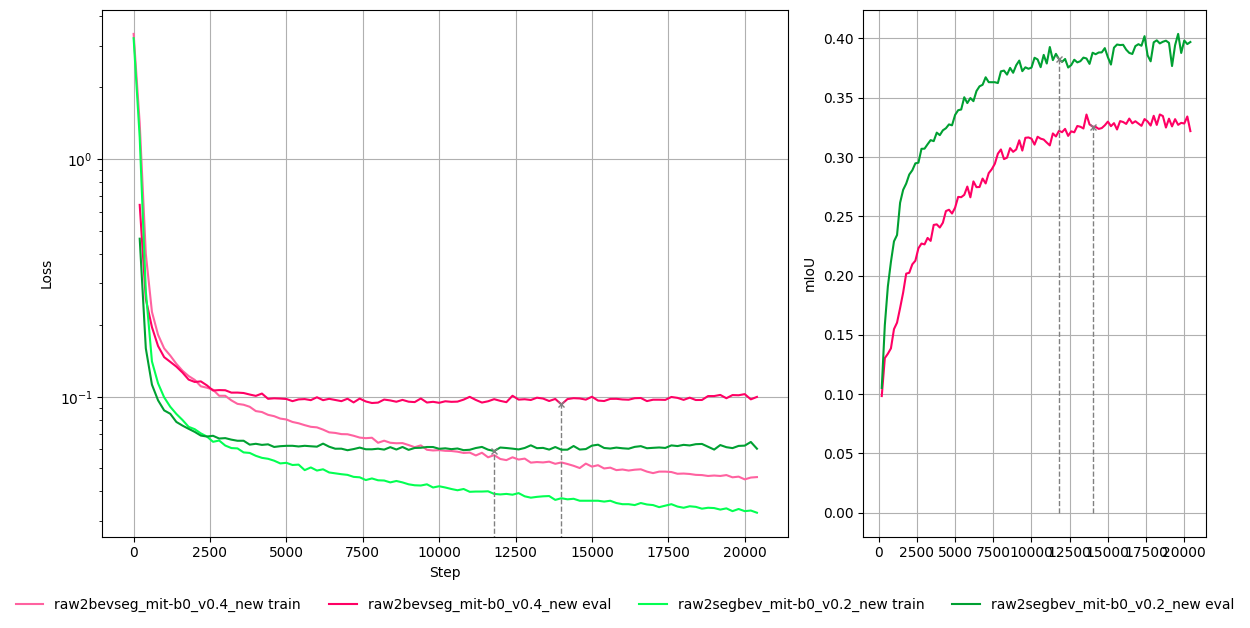
\includegraphics[width=0.7\linewidth]{./images/experiments/overfitting_bev_nu.png}
    \caption{Training and evaluation loss of raw2segbev and raw2bevseg MiT-b0 models without any regularization technique}
    \label{fig:overfitting_mit-b0}
\end{figure}

As shown in Figure~\ref{fig:overfitting_mit-b0}, both models showed clear signs of overfitting. While the training loss continued to decrease continuously, the validation loss began to increase, indicating a lack of generalization and failure to converge. These results highlight the importance of introducing regularization techniques even for small model sizes. Additionally, no signs of exploding gradients were observed during the training of these models. 

Two main approaches were selected to tackle the overfitting problem: weight decay (also known as L2 regularization) and data augmentation. Weight decay penalizes large weights during training, and makes the model more robust and less prone to memorizing irrelevant details; while data augmentation techniques introduces variability in the training dataset enabling the model to adapt better to unseen data. However, the introduction of data augmentation techniques into \aclink{BEV} images domain is not trivial and raises another research question wich is tackled in Section~\ref{sec:data_augmentation}.

It is also important to highlight the difference in metrics between the two models. Even though the backbone and training hyperparameters remain the same, there is a noticeable difference in both the loss values and the \aclink{mIoU} between the models. This difference is primarily due to the fact that the evaluation datasets differ. Specifically, the approach that segments the image first and then reprojects it is evaluated using semantic masks in the camera view, while the approach that first reprojects images into \aclink{BEV} and then performs segmentation is evaluated using masks directly in the \aclink{BEV} domain.

This distinction motivates the analysis shown in Figure~\ref{fig:normal_vs_bev_evaluation}, where the model \texttt{raw2segbev\_mit-b0\_v0.3} is evaluated on the test set twice: once using semantic masks in the camera domain and once using \aclink{BEV} masks. The figure displays the per-class \aclink{mIoU} for all the semantic categories the model was trained on, and two main observations emerge.

\begin{figure}[h!]
    \centering
    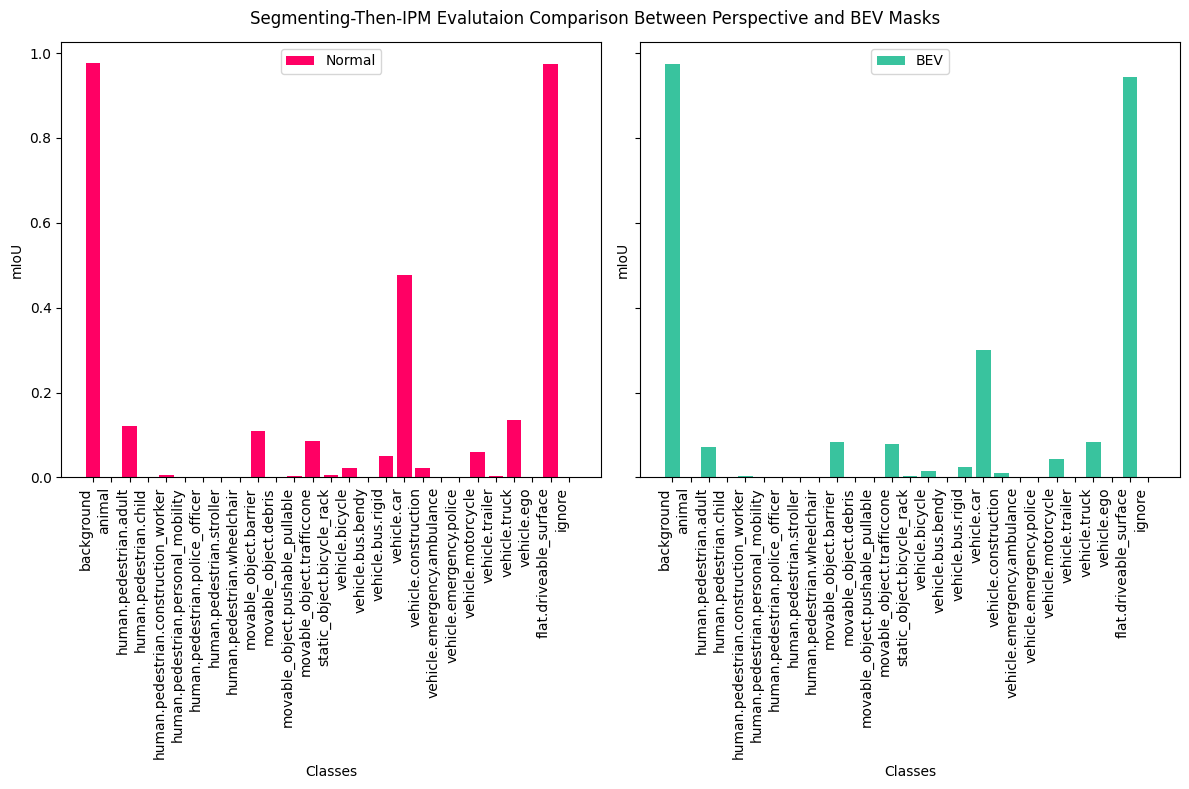
\includegraphics[width=0.8\linewidth]{./images/experiments/raw2segbev_mit-b0_v0.2_new_test_evaluation.png}
    \caption{Model evaluated with normal and BEV images}
    \label{fig:normal_vs_bev_evaluation}
\end{figure}

First, there's a clear imbalance in performance between dominant classes such as \texttt{background} and \texttt{flat.driveable\_area}, and the remaining, less frequent classes. Many of the minority classes show extremely low or even zero \aclink{IoU} scores. This is partly due to the inherent class imbalance in the dataset: some semantic classes have no annotated pixels at all (see Appendix~\ref{appendix:OLDatasets} for more details).

Second, all metrics are significantly higher when the model is evaluated using standard camera-domain masks. Reprojecting the masks to BEV introduces several effects: (1) a fixed background area appears in the BEV space that lies outside the camera's field of view; (2) the maximum scene distance is reduced to $30$ meters (see reprojection parameters in Section~\ref{sec:bev2seg_2}), which limits the presence of distant objects: minority classes like pedestrians are often excluded unless they are very close to the vehicle, while driveable areas and vehicles dominate the scene; and (3) the resolution is reduced to $1024 \times 1024$ pixels.

All these factors lead to a lower total number of pixels in the BEV dataset. As a result, each misclassified pixel has a greater impact on the overall evaluation, making errors more costly and consequently lowering the average performance metrics.

To address this, many training methods use class weighting in the loss function to penalize misclassifications of minority classes more heavily than those of majority classes. However, in this particular project, it is not essential to maintain all class distinctions provided by the dataset. Therefore, we investigate whether merging semantic classes can help mitigate the effects of class imbalance.

With all of this in place, the training strategy is designed to support experimentation in order to answer three main research questions:

\begin{itemize}
    \item \textit{Does the label's merging strategy helps increasing the model's performance on the low presence classes?}
    \item \textit{Which data augmentation technique is more effective for trainig a model directly on \aclink{BEV} images on a semantic segmentation task?}
    \item \textit{Which of the two approaches performs better for BEV driveable area segmentation?}
\end{itemize}

\hl{Mention the used hyperparameters for training the models.}

\subsubsection{Merging labels} \label{sec:merging_labels}
As previously discussed, to improve model performance on the dataset’s minority classes, a semantic label merging strategy was applied. This approach combines less represented semantic classes into more general, representative categories. Notably, this same merging strategy was already used in the annotation pipeline, so it was incorporated during training using the same look-up table of merging rules described in Table 3. The training and evaluation scripts were adapted accordingly to apply the merging rules consistently.

Table~\ref{tab:merging_comparison_bev} shows the results of two models trained with camera-perspective images and evaluated on the same test set using \aclink{BEV} masks. Model A was trained using the full set of original semantic classes, while Model B was trained using the merged classes, thereby reducing the total number of labels. 

In general, the results indicate that both models achieve comparable performance on the majority classes, specifically \texttt{background} and \texttt{flat.driveable\_surface}. However, a significant difference is observed in the minority classes, where Model B outperforms Model A across all evaluation metrics. This suggests that simplifying the semantic space does not decrease the model's ability to identify important instances and, instead, it reduces the penalty from underrepresented classes. Additionally, by reducing the number of classes, the overall average of the metrics improves as it avoids dilution from irrelevant or sparsely populated classes. This makes label merging especially useful in cases where fine-grained segmentation isn't necessary and consistency across the whole model is more important.

\begin{table}[h]
    \centering
    \tiny
    \begin{tabular}{llcccc}
    \toprule
    \textbf{Merged Class} & \textbf{Original Label} & \textbf{mIoU A} & \textbf{mIoU B} & \textbf{mF1 A} & \textbf{mF1 B} \\
    \midrule
    background & background & 0.97 & 0.97 & 0.99 & 0.99 \\
    \midrule
    animal & animal & 0.00 & 0.00 & 0.00 & 0.00 \\
    \midrule
    human.pedestrian.adult & human.pedestrian.adult & 0.07 & 0.08 & 0.09 & 0.11 \\
     & human.pedestrian.child & 0.00 & - & 0.00 & - \\
     & human.pedestrian.construction\_worker & 0.00 & - & 0.00 & - \\
     & human.pedestrian.personal\_mobility & 0.00 & - & 0.00 & - \\
     & human.pedestrian.police\_officer & 0.00 & - & 0.00 & - \\
     & human.pedestrian.stroller & 0.00 & - & 0.00 & - \\
     & human.pedestrian.wheelchair & 0.00 & - & 0.00 & - \\
    \midrule
    movable\_object.barrier & movable\_object.barrier & 0.08 & 0.14 & 0.09 & 0.17 \\
     & movable\_object.debris & 0.00 & - & 0.00 & - \\
     & movable\_object.pushable\_pullable & 0.00 & - & 0.00 & - \\
     & movable\_object.trafficcone & 0.08 & - & 0.10 & - \\
     & static\_object.bicycle\_rack & 0.00 & - & 0.00 & - \\
    \midrule
    vehicle.car & vehicle.bus.bendy & 0.00 & - & 0.00 & - \\
     & vehicle.bus.rigid & 0.02 & - & 0.03 & - \\
     & vehicle.car & 0.30 & 0.38 & 0.33 & 0.42 \\
     & vehicle.construction & 0.01 & - & 0.01 & - \\
     & vehicle.emergency.ambulance & 0.00 & - & 0.00 & - \\
     & vehicle.emergency.police & 0.00 & - & 0.00 & - \\
     & vehicle.trailer & 0.00 & - & 0.00 & - \\
     & vehicle.truck & 0.08 & - & 0.09 & - \\
    \midrule
    vehicle.ego & vehicle.ego & 0.00 & 0.00 & 0.00 & 0.00 \\
    \midrule
    vehicle.motorcycle & vehicle.bicycle & 0.02 & - & 0.02 & - \\
     & vehicle.motorcycle & 0.04 & 0.06 & 0.05 & 0.07 \\
    \midrule
    flat.driveable\_surface & flat.driveable\_surface & 0.94 & 0.94 & 0.97 & 0.97 \\
    \bottomrule
     & & 0.10 & 0.32 & 0.11 & 0.34 \\
    \bottomrule
    \end{tabular}
    \caption{Per-class metric comparison between Model A and merged Model B evaluated with BEV images}
    \label{tab:merging_comparison_bev}
\end{table}
    



\subsubsection{Data augmentation} \label{sec:data_augmentation}
Data augmentations are commonly used in deep learning models to mitigate overfitting during training and improve model generalization. There exists multiple types of data augmentation on the image domain: from pixel-based transformations, such as color space modifications, histogram equalization or filtering operations; to geometric transformations, including translations, rotations, shearings and homographies. These techniques have been widely applied in computer vision tasks and have shown to enhance model performance. However, performing data augmentation in \aclink{BEV} is not an easy task, as \aclink{IPM} images are already homographies of camera images, resulting in inherent distorsions.

Filtering operations can be applied to both standard and \aclink{BEV} images but geometric transformations were selected as the primary data augmentation method for camera domain images following the strategies employed in training the SegFormer model \cite{segformer}. Accordingly, random resizing, random cropping, and horizontal flipping were chosen as augmentation operations for perspective images.

Regarding \aclink{BEV} data augmentations, some multi-view methods implement strategies such as random flipping and random scaling, while others operate in the frequency domain \cite{HSDA}. However, these approaches apply augmentations to perspective images before the BEV transformation. Performing random cropping on a \aclink{BEV} image may lead to significant information loss, as large portions of the image may consist of unlabeled background data, potentially resulting in crops with insufficient information for effective training (Figure~\ref{fig:bev_cropping}). 

\begin{figure}[h]
    \centering
    % Row labels
    \setlength{\tabcolsep}{1pt}  % Reduce column padding
    \renewcommand{\arraystretch}{0.5}
    \begin{tabular}{c c c c c c c c}

        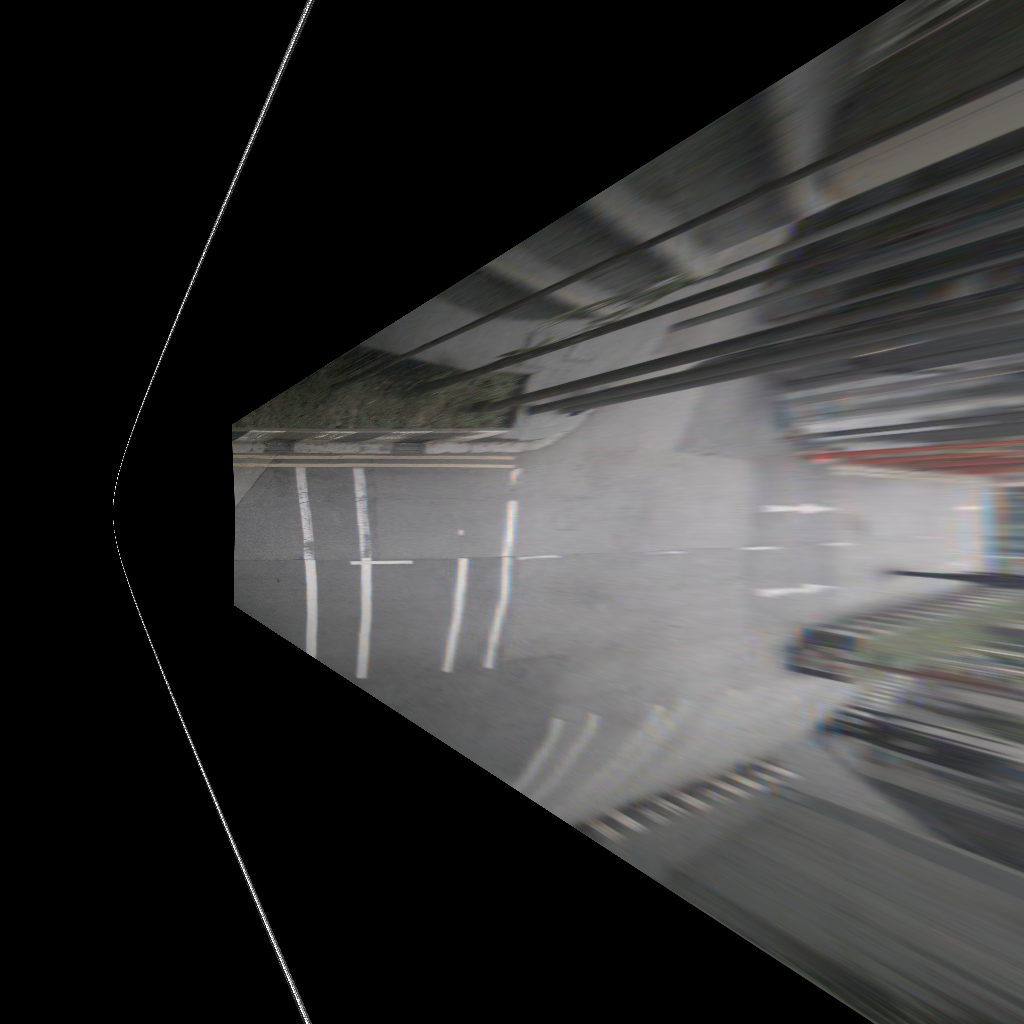
\includegraphics[width=0.12\textwidth]{images/methodology/mini/mini_0_bev.png} & 
        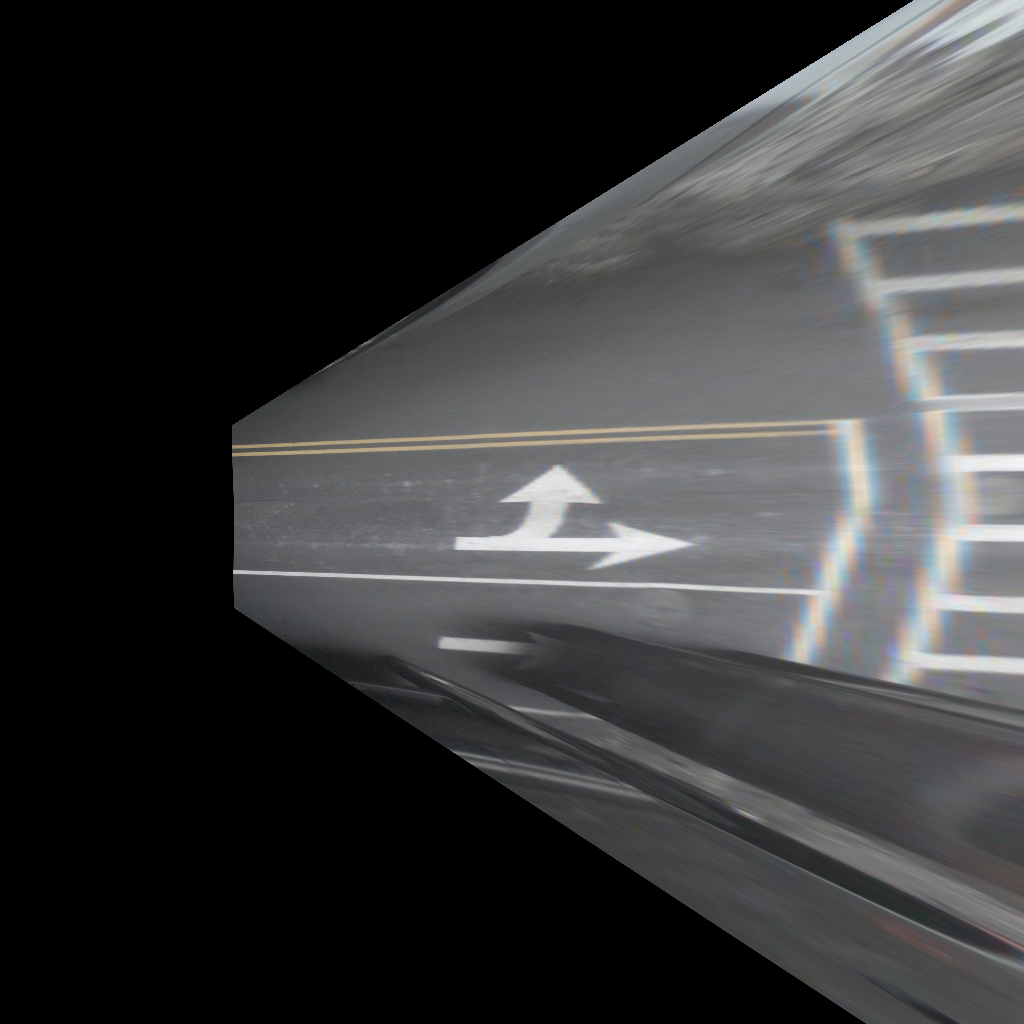
\includegraphics[width=0.12\textwidth]{images/methodology/mini/mini_1_bev.png} & 
        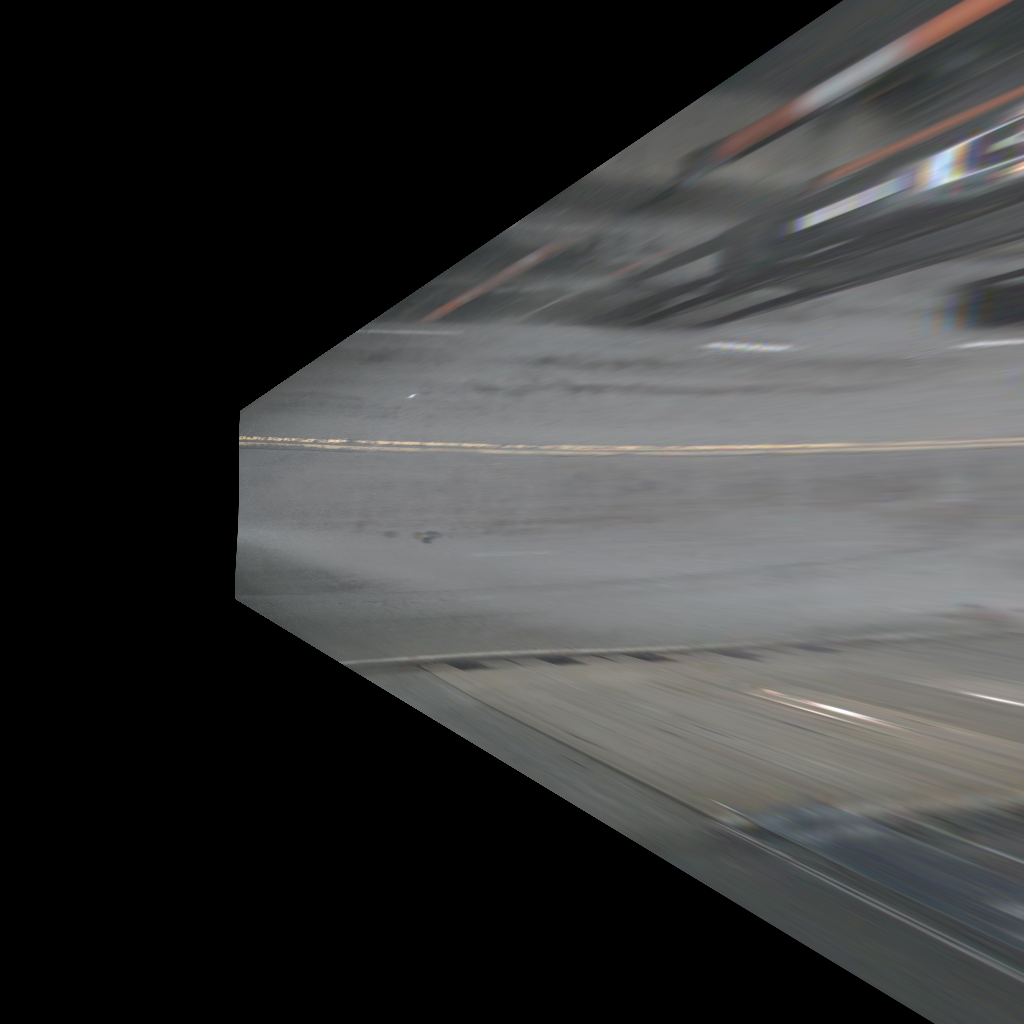
\includegraphics[width=0.12\textwidth]{images/methodology/mini/mini_2_bev.png} &
        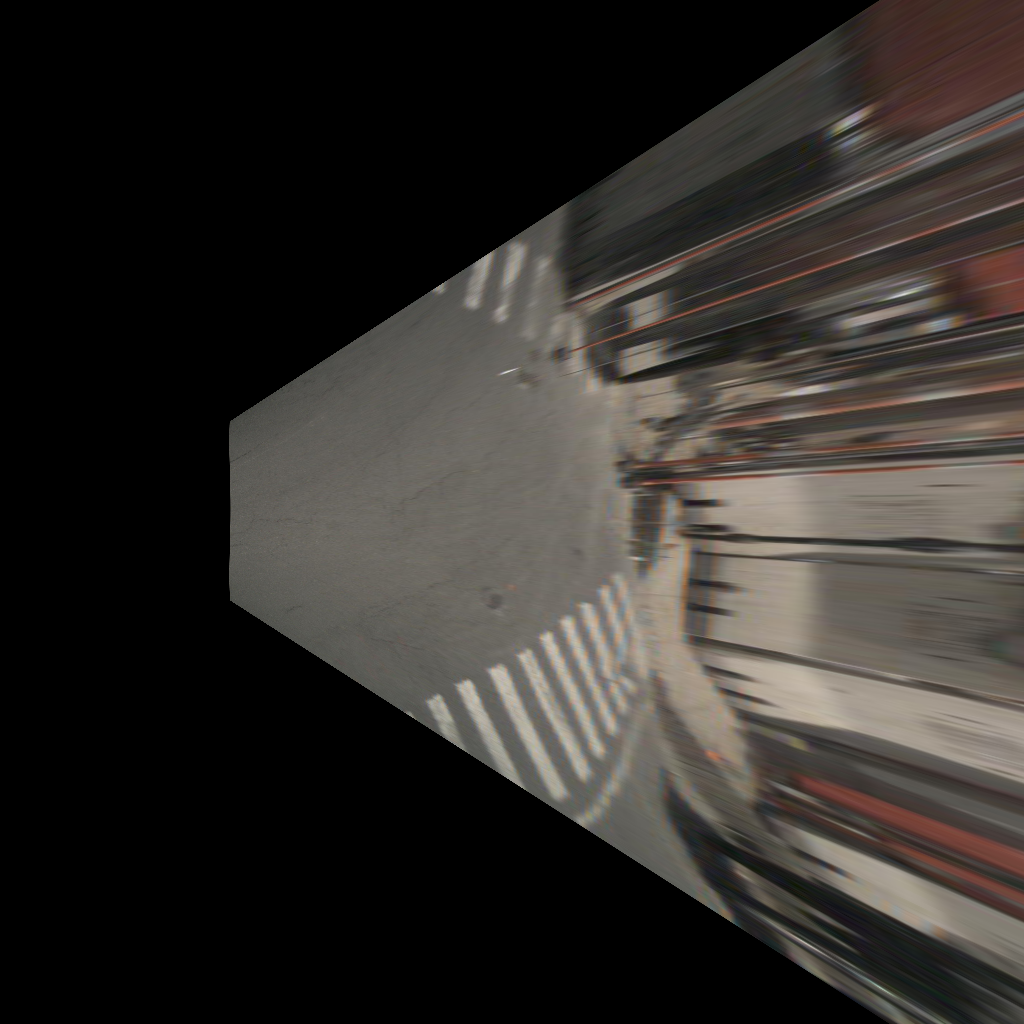
\includegraphics[width=0.12\textwidth]{images/methodology/mini/mini_3_bev.png} & 
        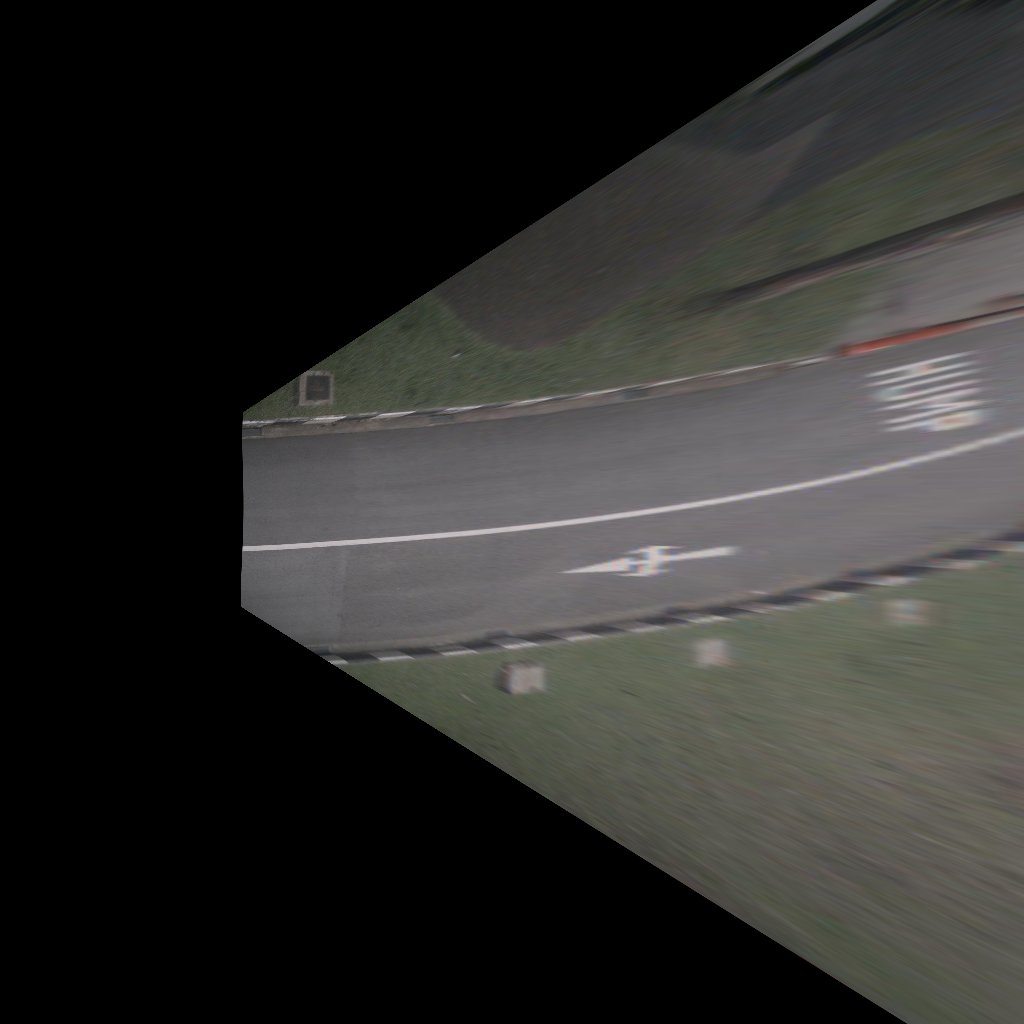
\includegraphics[width=0.12\textwidth]{images/methodology/mini/mini_4_bev.png} & 
        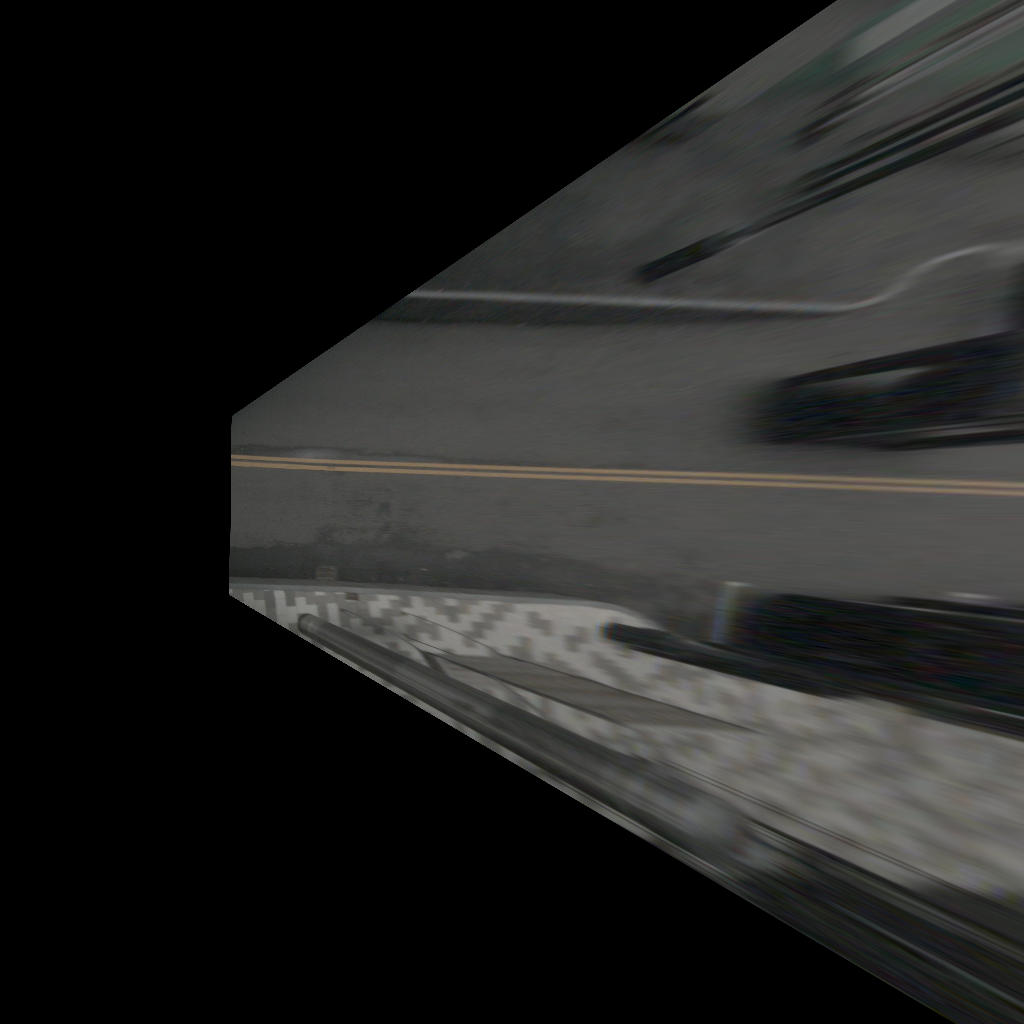
\includegraphics[width=0.12\textwidth]{images/methodology/mini/mini_5_bev.png} &
        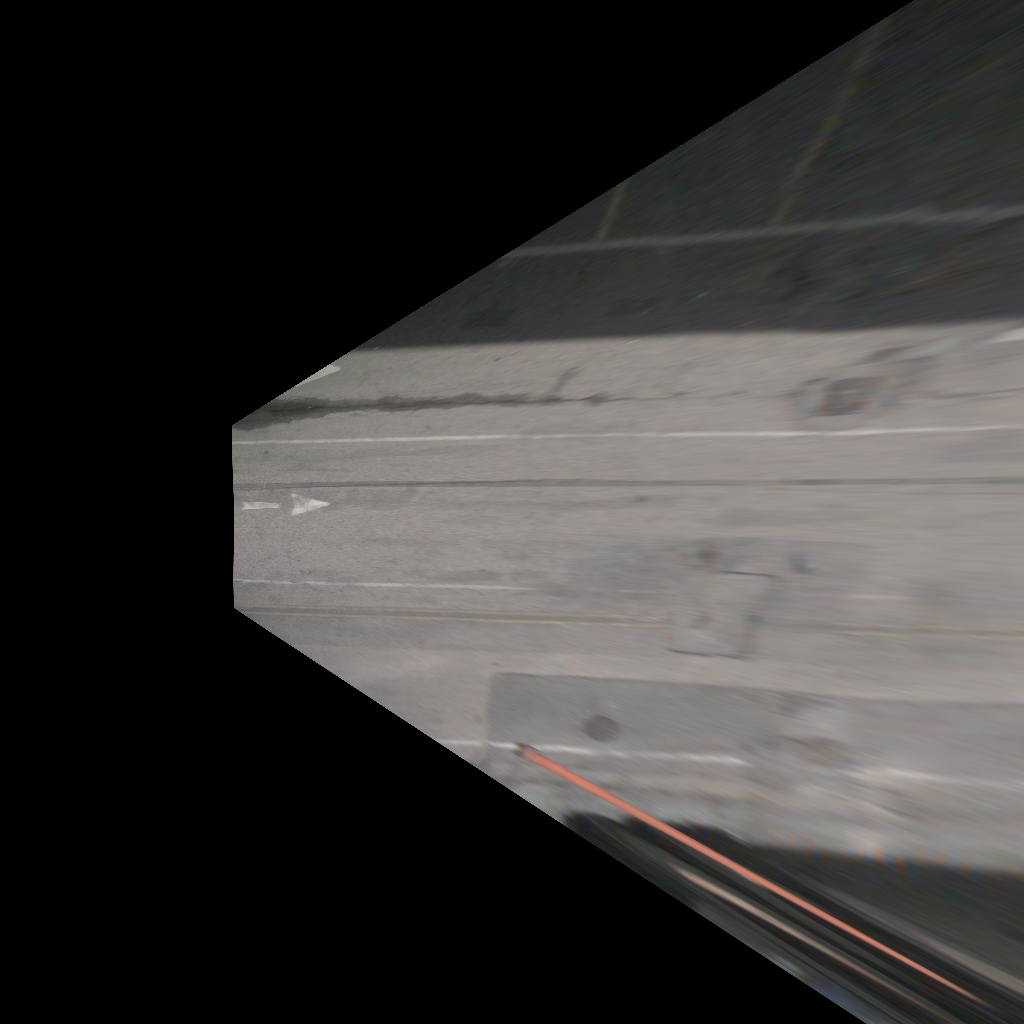
\includegraphics[width=0.12\textwidth]{images/methodology/mini/mini_6_bev.png} &
        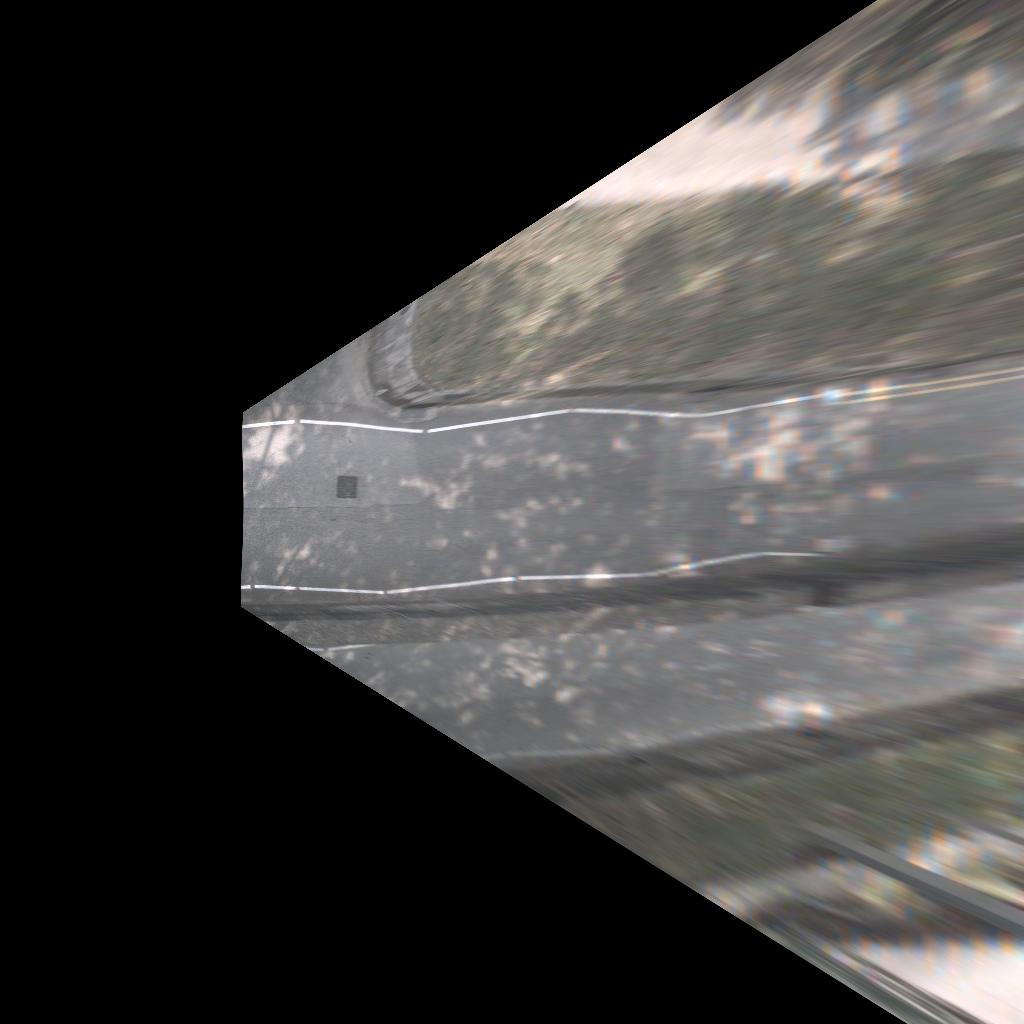
\includegraphics[width=0.12\textwidth]{images/methodology/mini/mini_7_bev.png} \\ 
        
        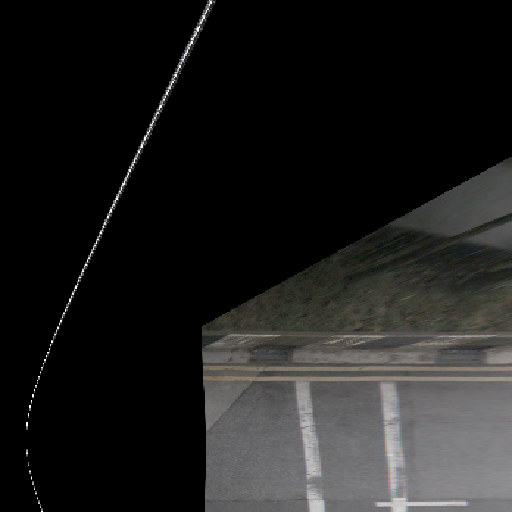
\includegraphics[width=0.12\textwidth]{images/methodology/data_augmentations/bev_crop_image_0_9.png} & 
        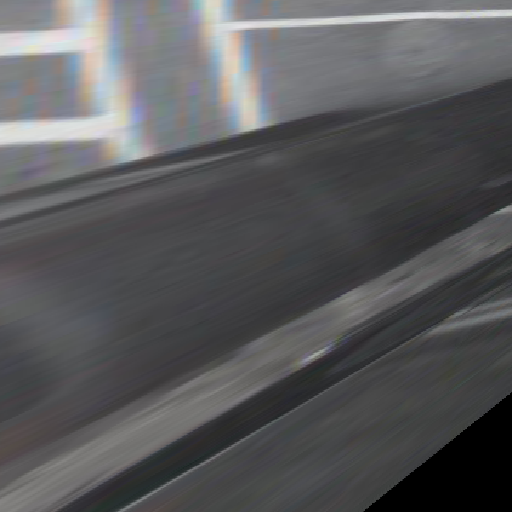
\includegraphics[width=0.12\textwidth]{images/methodology/data_augmentations/bev_crop_image_1_2.png} & 
        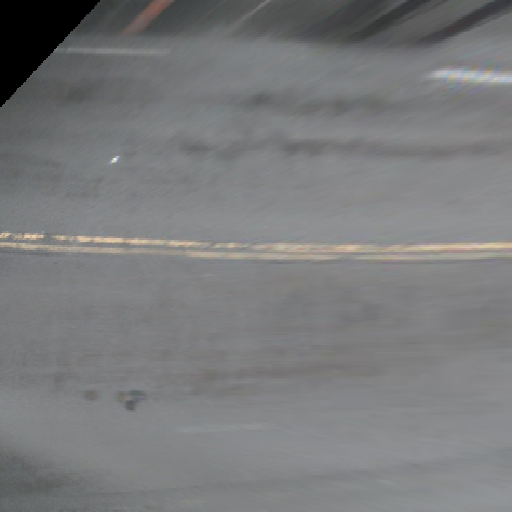
\includegraphics[width=0.12\textwidth]{images/methodology/data_augmentations/bev_crop_image_2_5.png} &
        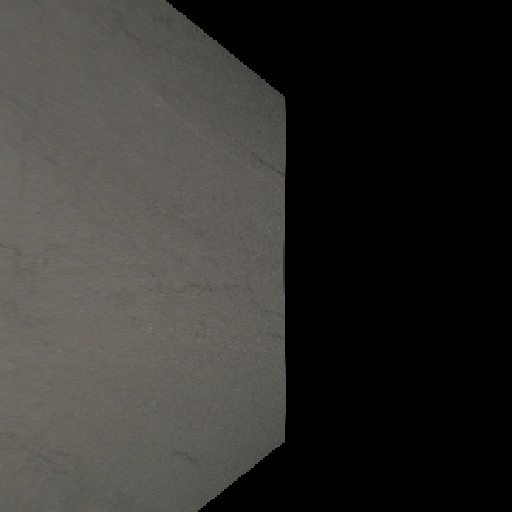
\includegraphics[width=0.12\textwidth]{images/methodology/data_augmentations/bev_crop_image_3_5.png} & 
        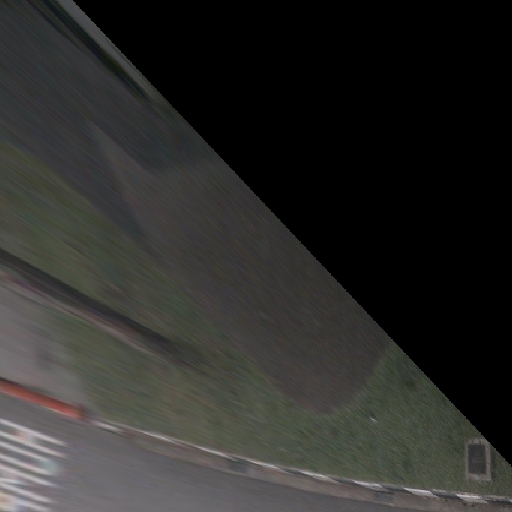
\includegraphics[width=0.12\textwidth]{images/methodology/data_augmentations/bev_crop_image_4_3.png} & 
        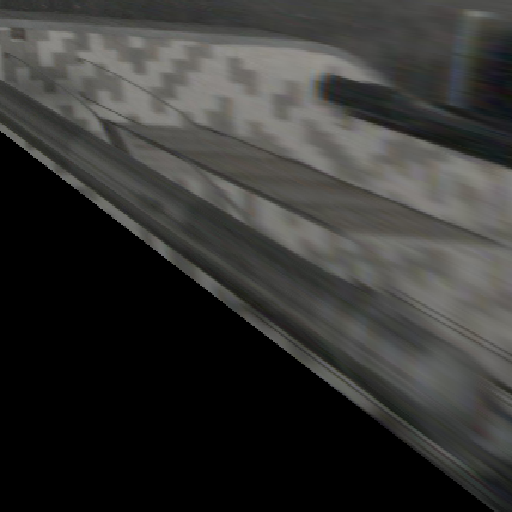
\includegraphics[width=0.12\textwidth]{images/methodology/data_augmentations/bev_crop_image_5_2.png} &
        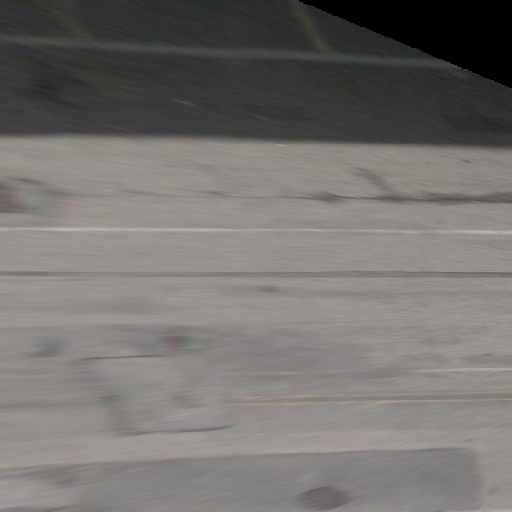
\includegraphics[width=0.12\textwidth]{images/methodology/data_augmentations/bev_crop_image_6_1.png} &
        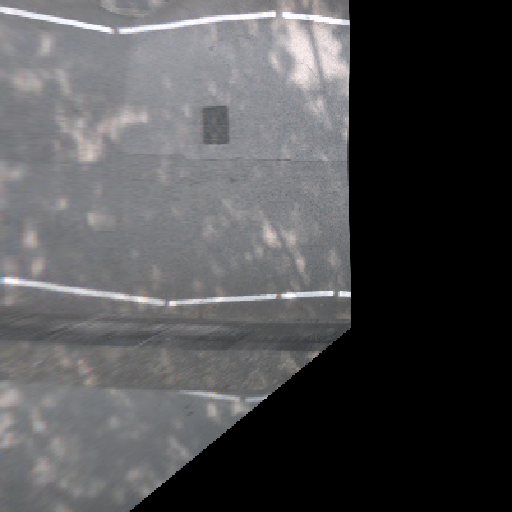
\includegraphics[width=0.12\textwidth]{images/methodology/data_augmentations/bev_crop_image_7_2.png} \\ 

        
\includegraphics[width=0.12\textwidth]{images/methodology/data_augmentations/bev_crop_mask_0_9.png} & 
        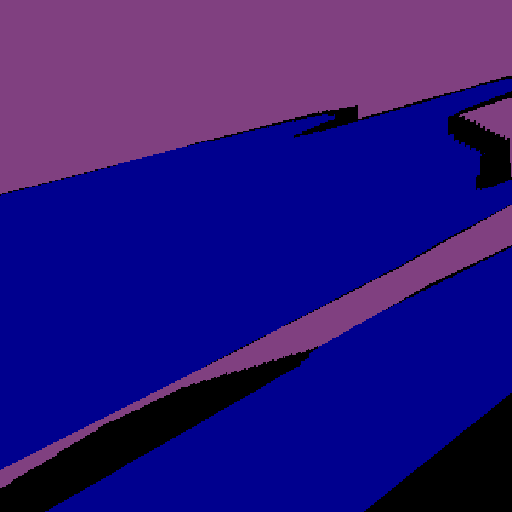
\includegraphics[width=0.12\textwidth]{images/methodology/data_augmentations/bev_crop_mask_1_2.png} & 
        
\includegraphics[width=0.12\textwidth]{images/methodology/data_augmentations/bev_crop_mask_2_5.png} &
        
\includegraphics[width=0.12\textwidth]{images/methodology/data_augmentations/bev_crop_mask_3_5.png} & 
        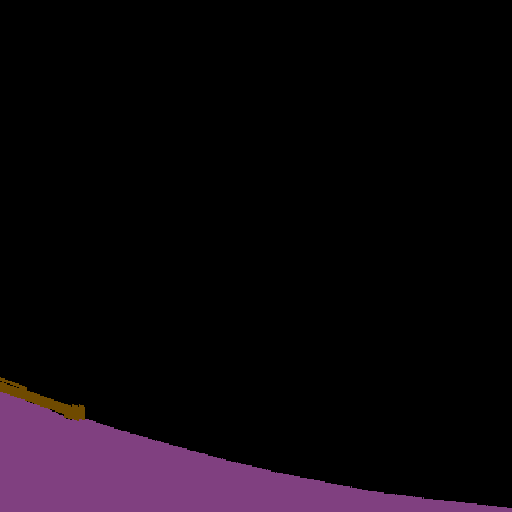
\includegraphics[width=0.12\textwidth]{images/methodology/data_augmentations/bev_crop_mask_4_3.png} & 
        
\includegraphics[width=0.12\textwidth]{images/methodology/data_augmentations/bev_crop_mask_5_2.png} &
        
\includegraphics[width=0.12\textwidth]{images/methodology/data_augmentations/bev_crop_mask_6_1.png} &
        
\includegraphics[width=0.12\textwidth]{images/methodology/data_augmentations/bev_crop_mask_7_2.png} \\

    \end{tabular}
    
    \caption{Random cropping and horizontal flipping on BEV images. Original BEV images on first row; random flipped and cropped images on second row and corresponding semantic masks on last row.}
    \label{fig:bev_cropping}
\end{figure}

In this context, a different approach was also considered: applying geometric transformations by modifying the camera's extrinsic parameters before reprojecting to \aclink{BEV} space. The objective is to introduce random transformations along one of the camera’s rotation axes, generating diverse \aclink{BEV} reprojections with varying degrees of distortion. This technique may enable the model to adapt to different extrinsic camera configurations, improving its robustness to variations in camera placement and orientation (Figure~\ref{fig:bev_data_aug}).

\begin{figure}[h]
    \centering
    % Row labels
    \setlength{\tabcolsep}{1pt}  % Reduce column padding
    \renewcommand{\arraystretch}{0.5}
    \begin{tabular}{c c c c c c}
        & $-0.25$ rad & $-0.125$ rad & $0.0$ rad & $0.125$ rad & $0.25$ rad \\ 
        
        \rotatebox{90}{\textbf{Yaw}} & 
        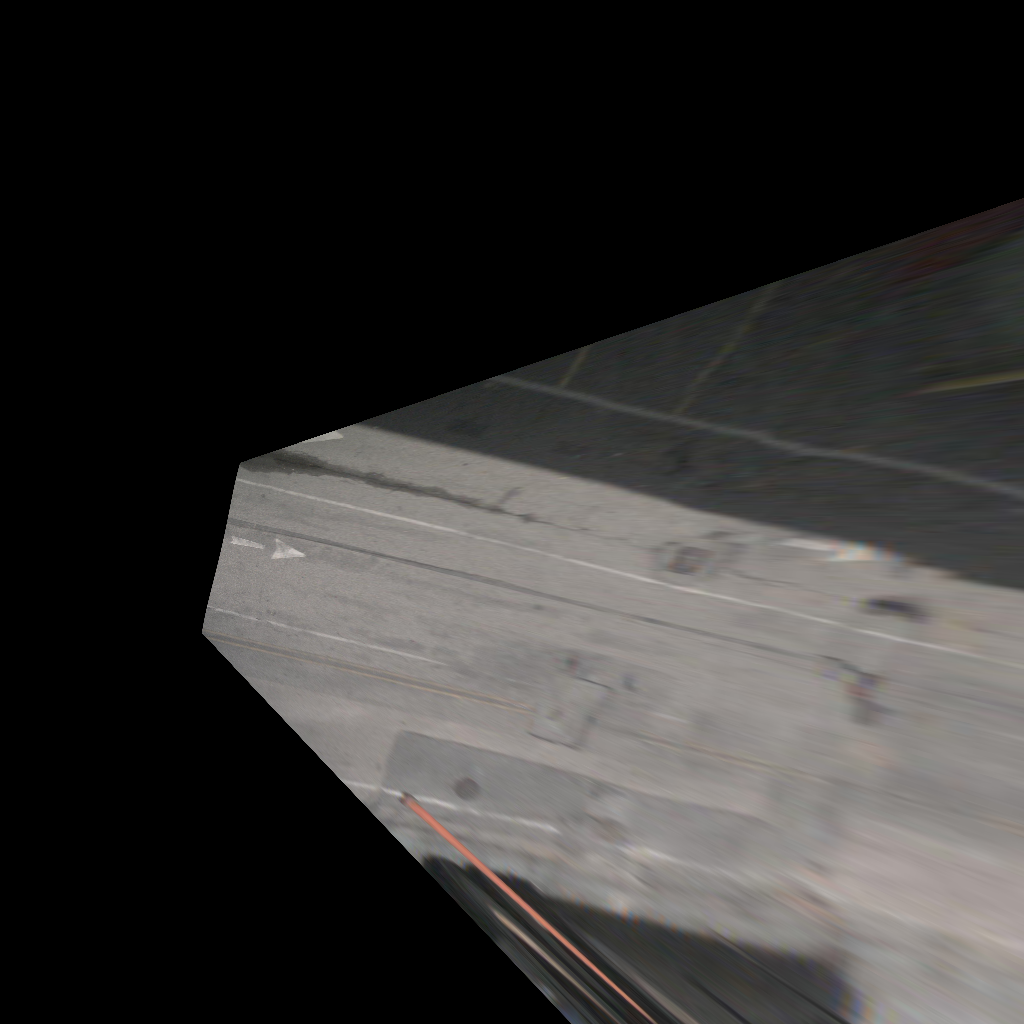
\includegraphics[width=0.15\textwidth]{images/methodology/data_augmentations/rx_-0.25_0.png} & 
        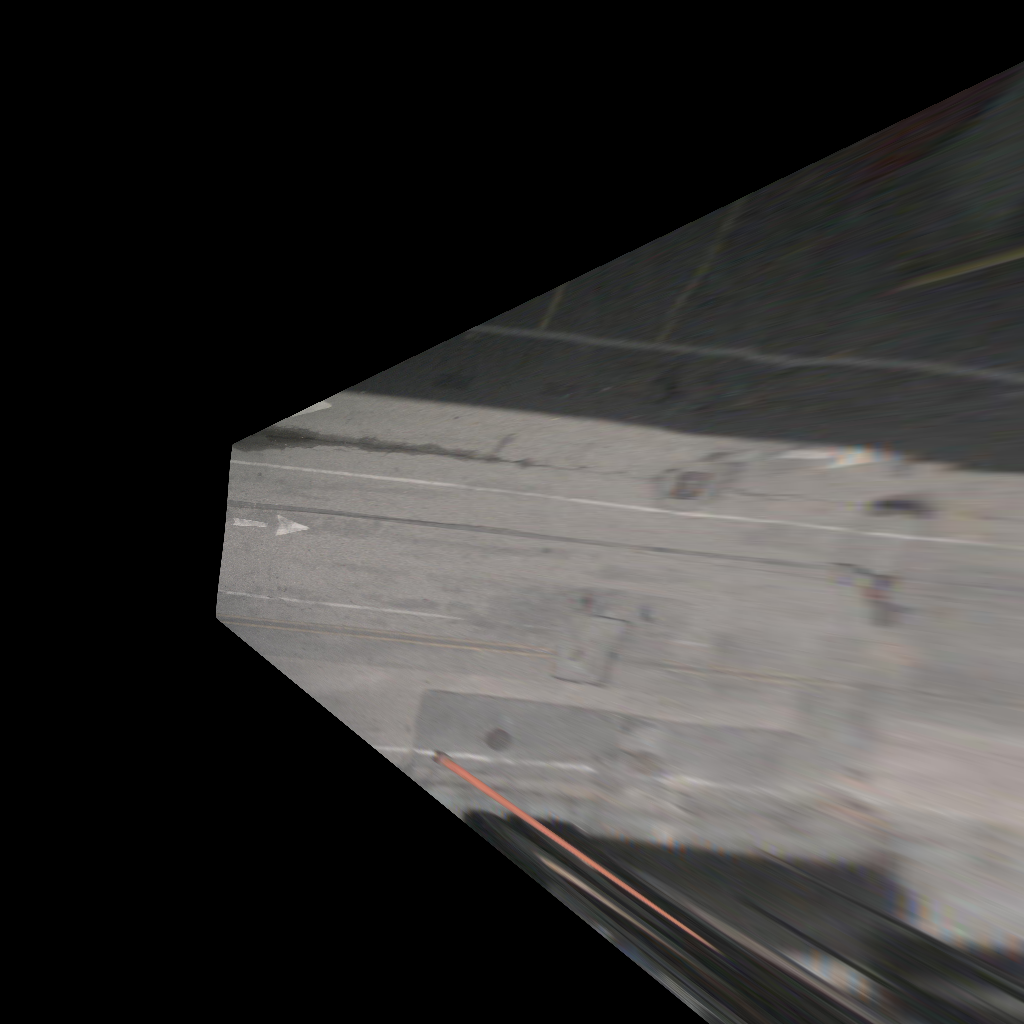
\includegraphics[width=0.15\textwidth]{images/methodology/data_augmentations/rx_-0.125_1.png} & 
        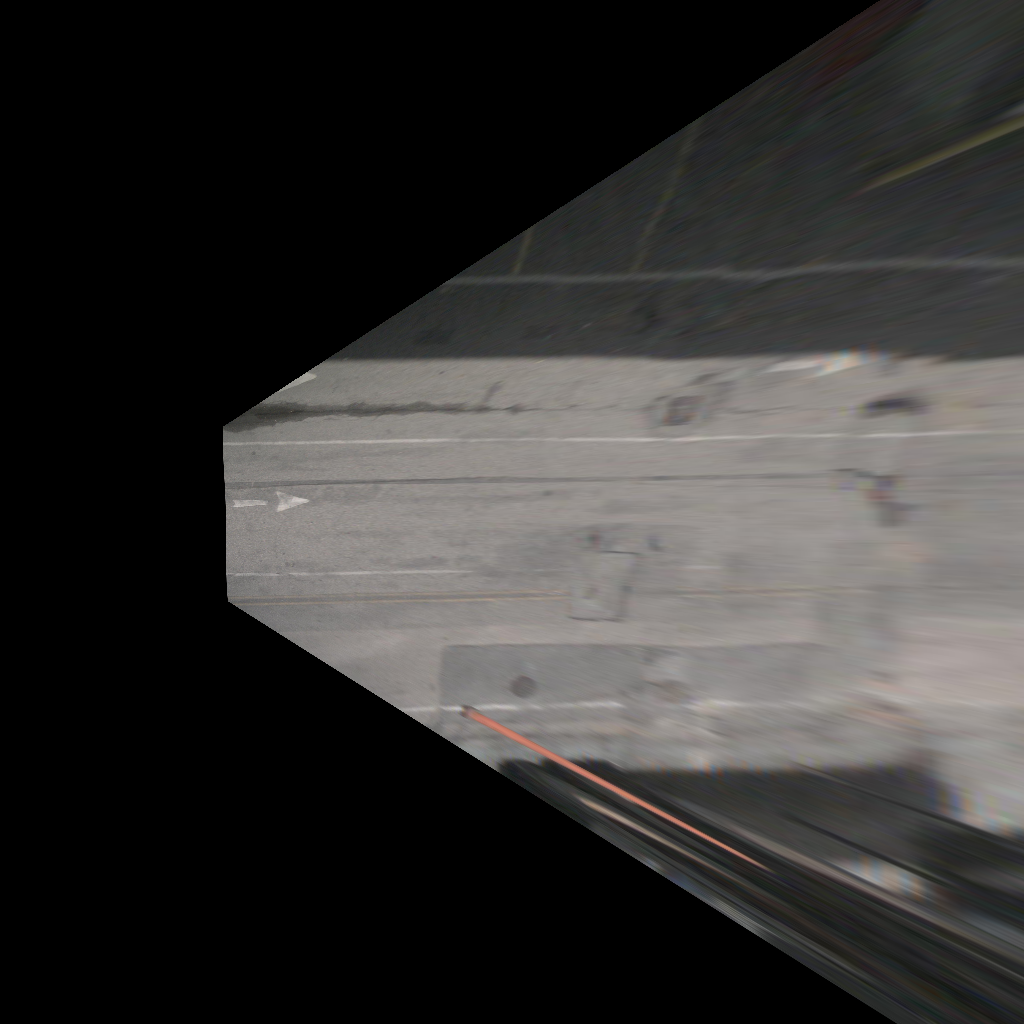
\includegraphics[width=0.15\textwidth]{images/methodology/data_augmentations/rx_0.0_2.png} & 
        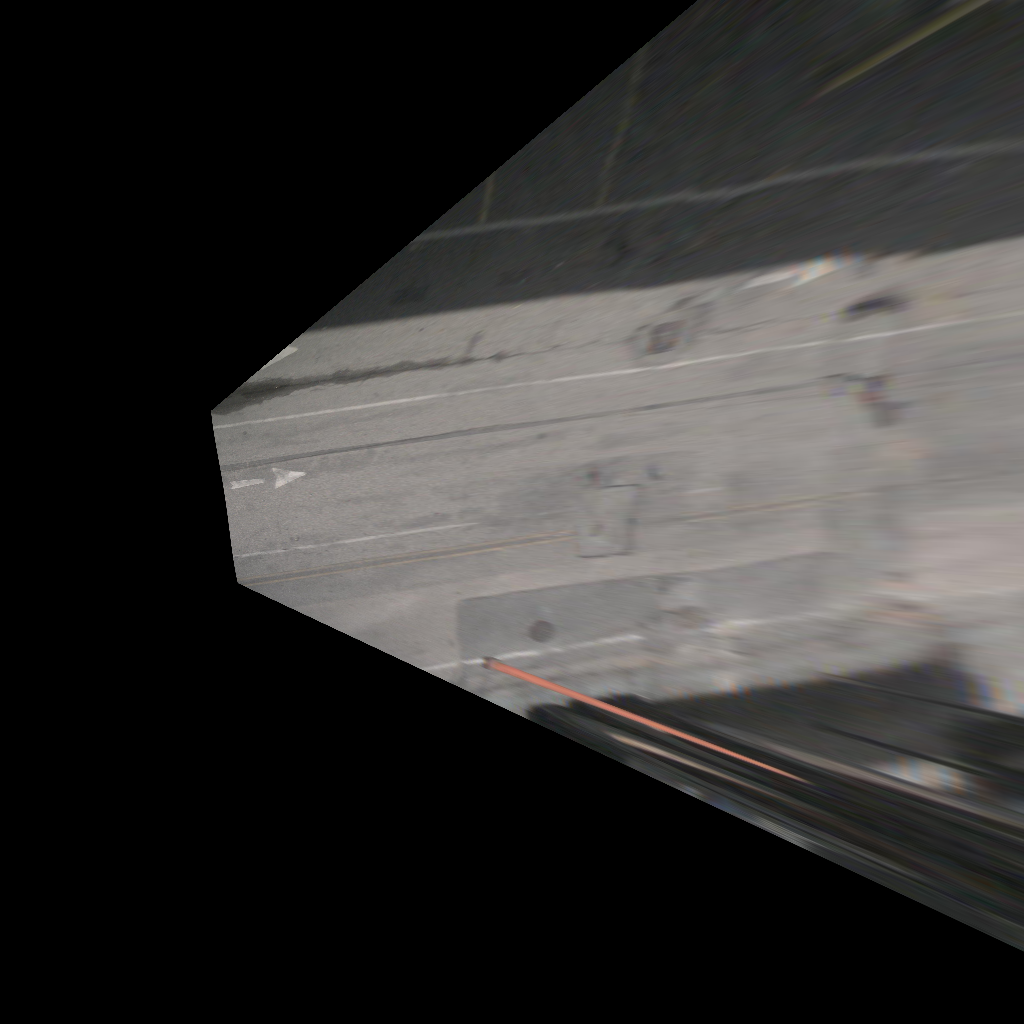
\includegraphics[width=0.15\textwidth]{images/methodology/data_augmentations/rx_0.125_3.png} & 
        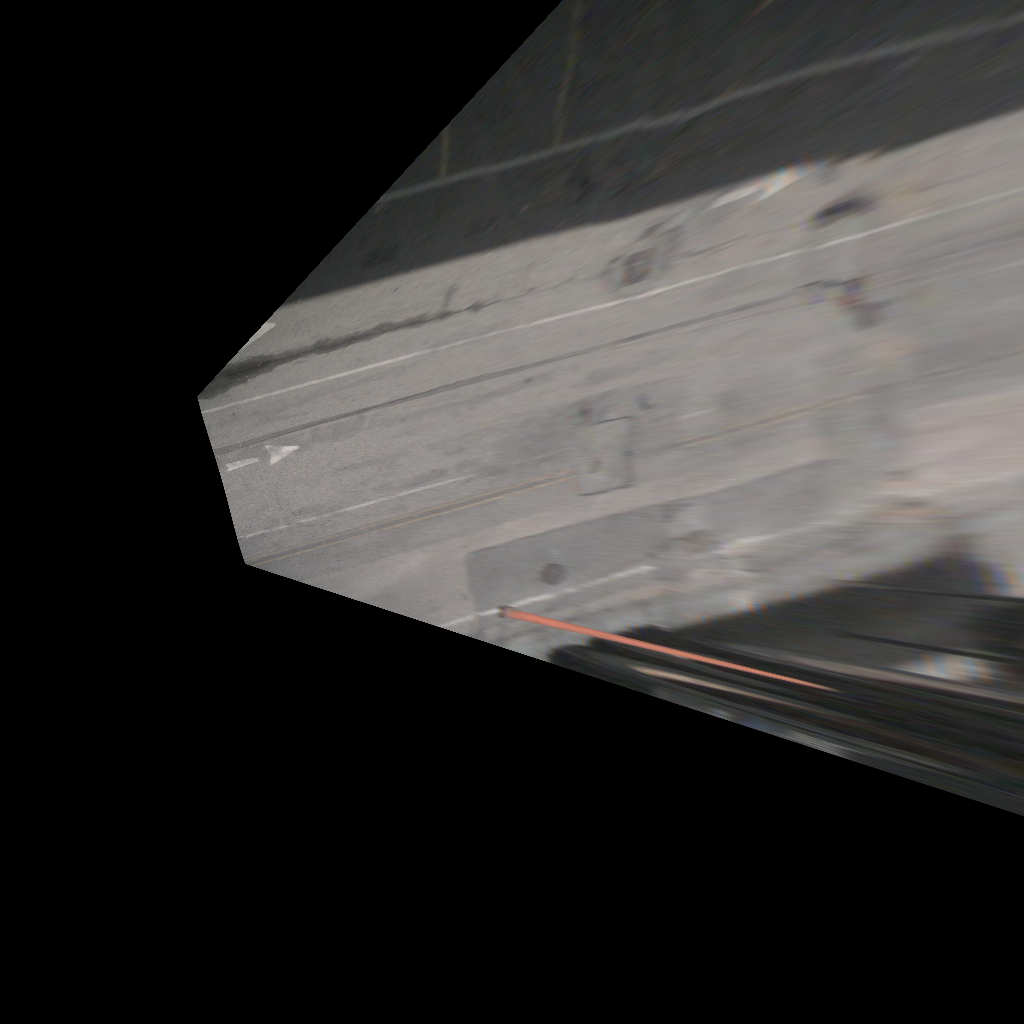
\includegraphics[width=0.15\textwidth]{images/methodology/data_augmentations/rx_0.25_4.png} \\ 
        
        \rotatebox{90}{\textbf{Pitch}} & 
        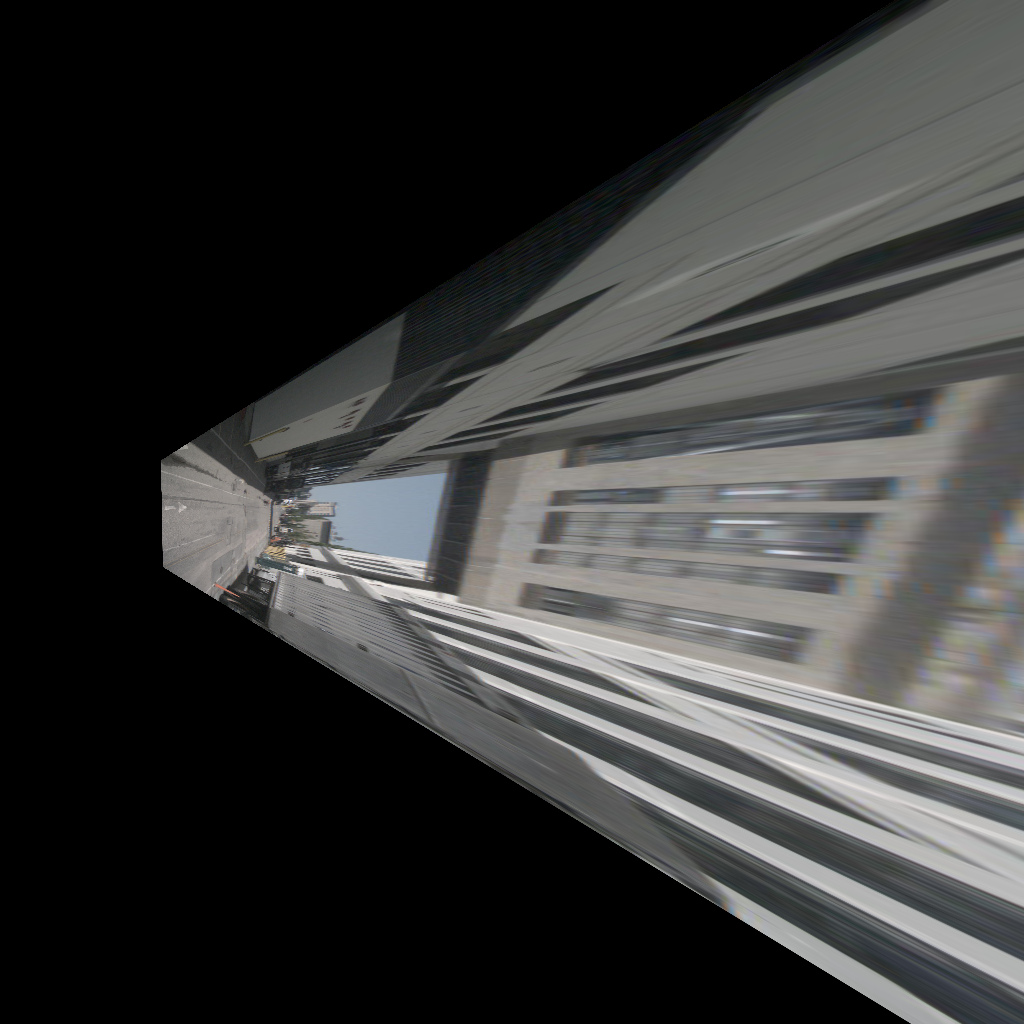
\includegraphics[width=0.15\textwidth]{images/methodology/data_augmentations/rz_-0.25_0.png} & 
        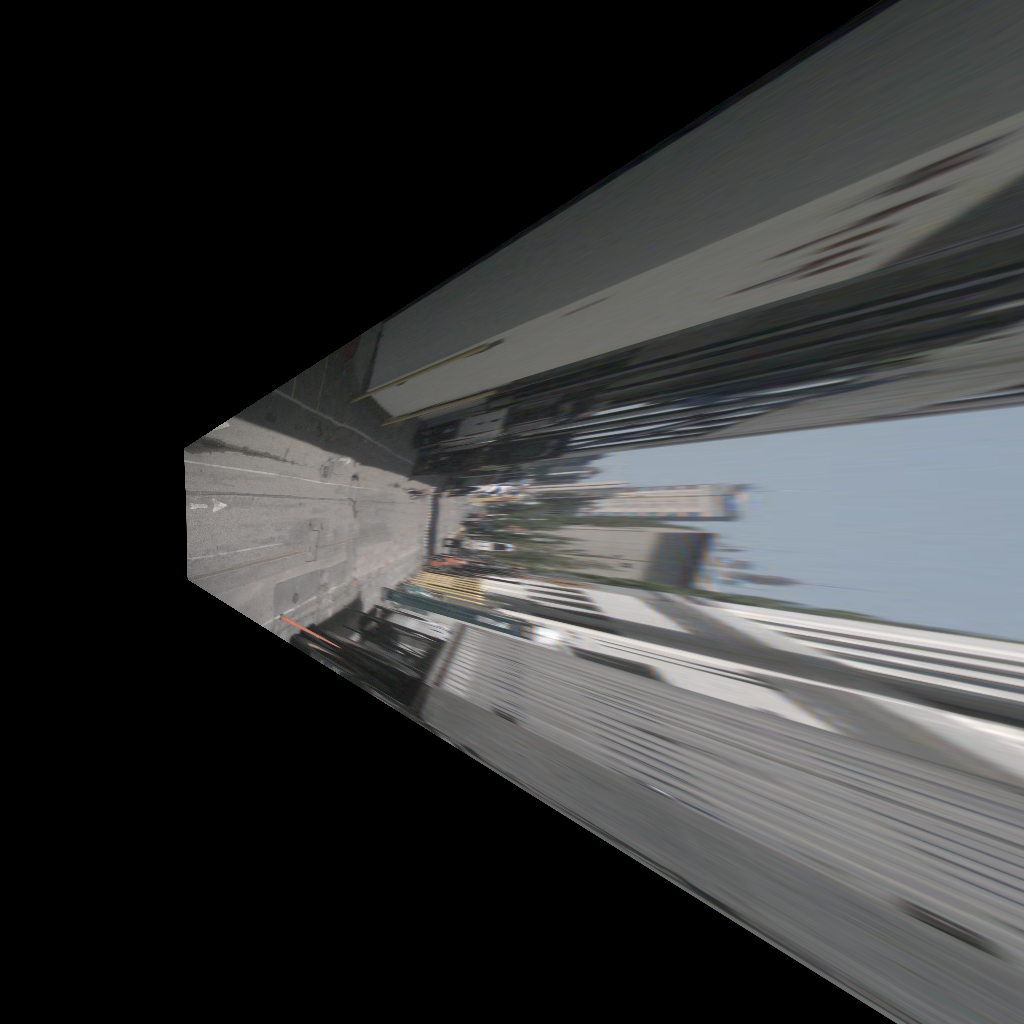
\includegraphics[width=0.15\textwidth]{images/methodology/data_augmentations/rz_-0.125_1.png} & 
        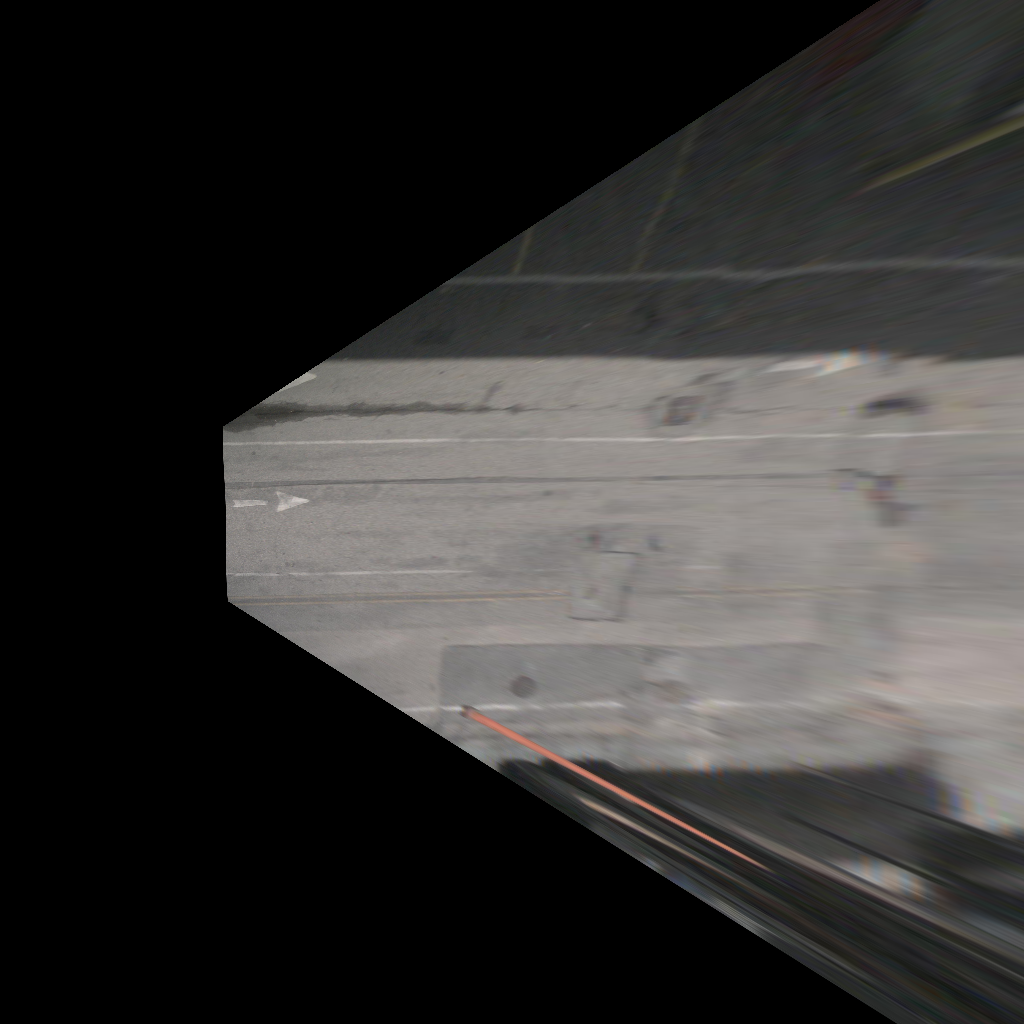
\includegraphics[width=0.15\textwidth]{images/methodology/data_augmentations/rz_0.0_2.png} & 
        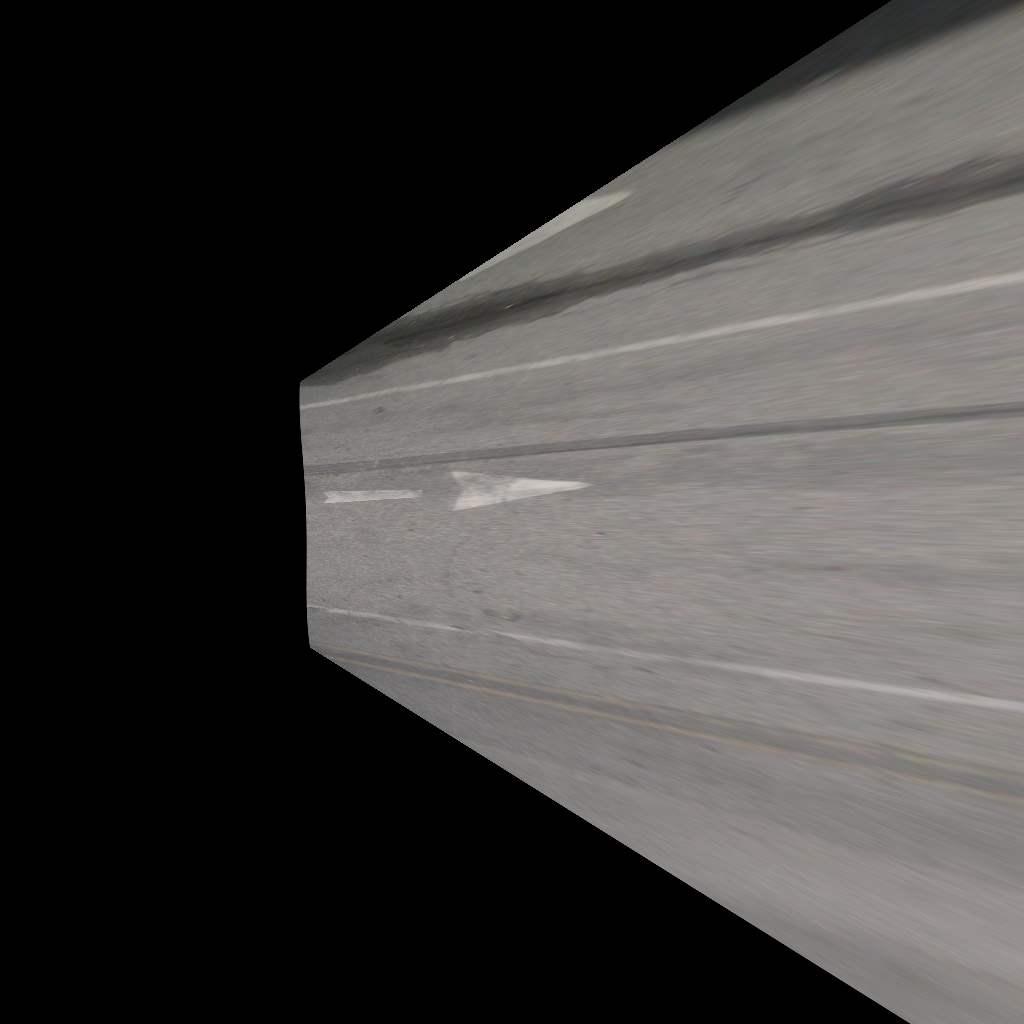
\includegraphics[width=0.15\textwidth]{images/methodology/data_augmentations/rz_0.125_3.png} & 
        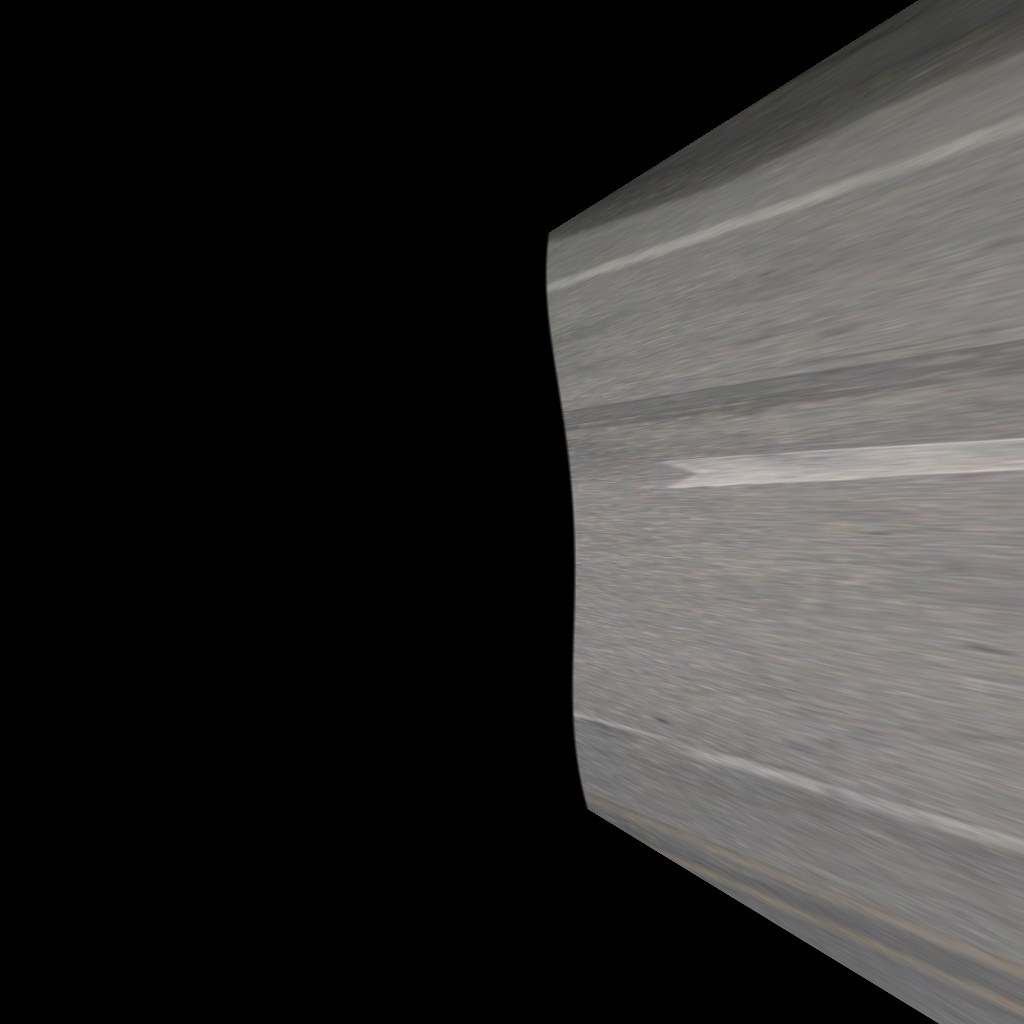
\includegraphics[width=0.15\textwidth]{images/methodology/data_augmentations/rz_0.25_4.png} \\ 

        \rotatebox{90}{\textbf{Roll}} & 
        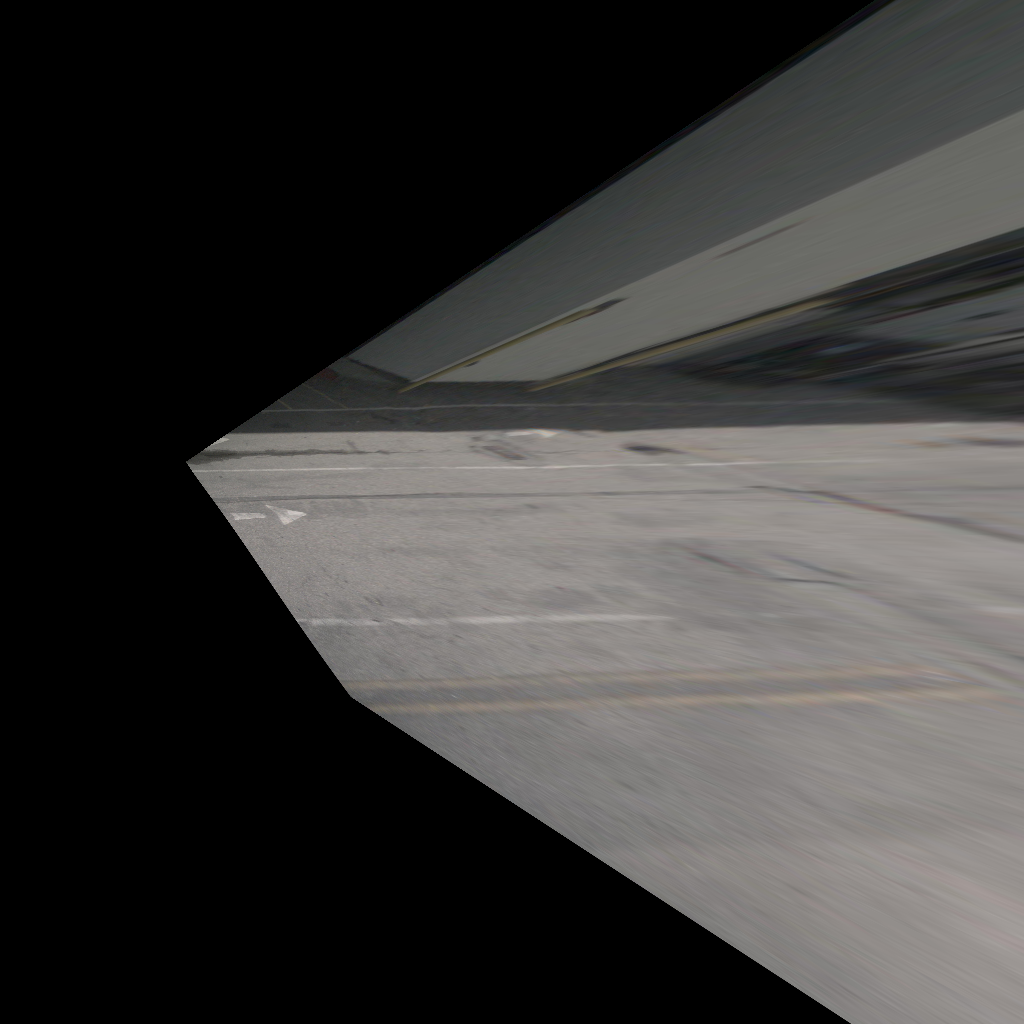
\includegraphics[width=0.15\textwidth]{images/methodology/data_augmentations/ry_-0.25_0.png} & 
        \includegraphics[width=0.15\textwidth]{images/methodology/data_augmentations/ry_-0.125_1.png} & 
        \includegraphics[width=0.15\textwidth]{images/methodology/data_augmentations/ry_0.0_2.png} & 
        \includegraphics[width=0.15\textwidth]{images/methodology/data_augmentations/ry_0.125_3.png} & 
        \includegraphics[width=0.15\textwidth]{images/methodology/data_augmentations/ry_0.25_4.png} \\ 
        
    \end{tabular}
    
    \caption{Effect of camera transformations on BEV projection. The first row shows variations in the yaw axes, the second in pitch, and the third in roll.}
    \label{fig:bev_data_aug}
\end{figure}


This section has a dual purpose. First, the effect of applying geometric transformations to camera-perspective images as data augmetation strategy for training a traditional segmentation model in order to mitigate overfitting is studied. Second, the effectiveness of two described techniques for performing data augmentation on \aclink{BEV} images is explored: applying the same geometric augmentations used for regular images, or modifying the camera's extrinsic parameters before performing the projections.

Therefore, the introduction of data augmentation strategies such as random cropping, horizontal flipping, and rescaling on regular images significantly reduces overfitting, as shown in Figure~\ref{fig:normal_before_after_data_aug_logs}. This reduction in overfitting allows for longer training periods and improves model performance on the evaluation set, leading to convergence at higher \aclink{mIoU} values. This effect is also reflected in the evaluation of the models on the test set, where the model with data augmentation presents higher \aclink{mIoU} than the model affected by overfitting.

\begin{figure}[h!]
    \centering
    \includegraphics[width=0.7\linewidth]{./images/experiments/nor_before_after_data_aug_logs.png}
    \caption{Before and after regularization techniques on models trained with camera-domain images}
    \label{fig:normal_before_after_data_aug_logs}
\end{figure}

Secondly, the Figure~\ref{fig:bev_before_after_data_aug_logs} shows the trainig process graph for the three models trained with \aclink{BEV} images and reveals some significant differences. The first model, without any data augmentation, exhibits notable overfitting. In contrast, both data augmentation strategies, the traditional geometric augmentations (random flipping, random cropping, and rescaling) and the custom strategy of modifying the camera's extrinsic parameters, seems to partially reduce this overfitting.

\begin{figure}[h!]
    \centering
    \includegraphics[width=0.7\linewidth]{./images/experiments/bev_before_after_data_aug_logs.png}
    \caption{Training logs of models with BEV data augmentation techniques}
    \label{fig:bev_before_after_data_aug_logs}
\end{figure}

Focusing on the model employing traditional data augmentation techniques on the BEV images, the training error is generally higher, and the training and validation error curves remain closely aligned with a considerably lower mIoU on the validation set compared to the other two models. This pattern suggests potential underfitting. This observation appears to support the initial hypothesis that directly applying traditional image augmentations to BEV representations might not provide the model with sufficiently informative variations for effective training in this specific domain.

On the other hand, the model trained with the extrinsic's data augmentation strategy shows less overfitting than the model without any data augmentation technique. This allows for more extended training and achieves superior results on the validation set, outperforming the overfitted model. 

Overall, the findings from the validation set suggest that the custom data augmentation techniques for BEV images offer better performance than directly applying traditional augmentations. However, it is crucial to examine the models' performance on the unseen test set. Figure~\ref{fig:bev_before_after_data_aug_test} illustrates this evaluation, revealing that the performance difference between the three models is not as substantial in reality. While the model trained with extrinsic's parameters modification shows slightly better results, the performance gap between the other two models is less clear, with the model using traditional data augmentation on BEV images occasionally surpassing the overfitted model in vehicle-related classes.

\begin{figure}[h!]
    \centering
    \includegraphics[width=0.7\linewidth]{./images/experiments/bev_before_after_data_aug_test.png}
    \caption{Different data augmentation stategies evaluated with BEV images.}
    \label{fig:bev_before_after_data_aug_test}
\end{figure}

\subsubsection{Segmenting-Then-IPM vs IPM-Then-Segmenting}
The Table~\ref{tab:model_comparison} shows a comparative analysis of semantic segmentation performance across different models, categorized into two distinct \aclink{BEV} mask generation pipelines: "\aclink{IPM} Then Segmenting" and "Segmenting Then \aclink{IPM}". Values represent the \aclink{mIoU} for the merged semantic classes (Section~\ref{sec:merging_labels}), with "Mean" indicating the average \aclink{mIoU} across all displayed classes for each model. Also, models are categorized by their architecture (MiT-B0, MiT-B2, MiT-B4) and the used data augmentation technique (O: No data augmentation, overfitted model; N: Normal data augmentation; E: Camera's extrinsic parameters modification)

\begin{table}[h]
    \centering

    \begin{threeparttable}
        \tiny
        \newcolumntype{C}[1]{>{\centering\arraybackslash}m{#1}}
        \begin{tabular}{l | C{0.7cm} C{1.3cm} C{1cm} C{1.2cm} C{1cm} C{0.7cm} C{0.7cm} C{1.3cm} | c}
            \toprule
            \textbf{Model} & \textbf{animal} & \textbf{background} & \textbf{\makecell{flat.\\driveable\\\textunderscore surface}} & \textbf{\makecell{human.\\pedestrian.\\adult}} & \textbf{\makecell{movable\\\textunderscore object.\\barrier}} & \textbf{\makecell{vehicle.\\car}} & \textbf{\makecell{vehicle.\\ego}} & \textbf{\makecell{vehicle.\\motorcycle}} & \textbf{Mean} \\
            \midrule

            \multicolumn{10}{l}{\textbf{IPM Then Segmenting}} \\
            \midrule
            \multirow{1}{*}{\text{MiT-B0 O}}  & 0.00 & 0.97 & 0.93 & 0.04 & 0.14 & 0.32 & 0.00 & 0.04 & 0.30 \\
            \multirow{1}{*}{\text{MiT-B0 E}}  & 0.00 & 0.97 & 0.94 & 0.04 & 0.14 & 0.34 & 0.00 & 0.04 & 0.31 \\
            \multirow{1}{*}{\text{MiT-B2 E}}  & 0.00 & 0.97 & 0.95 & 0.05 & 0.17 & 0.36 & 0.00 & 0.05 & 0.32 \\
            \multirow{1}{*}{\text{MiT-B4 E}}  & 0.00 & 0.98 & 0.95 & 0.06 & 0.17 & 0.36 & 0.00 & 0.06 & 0.32 \\
            \multirow{1}{*}{\text{MiT-B0 N}}  & 0.00 & 0.97 & 0.94 & 0.03 & 0.14 & 0.32 & 0.00 & 0.03 & 0.30 \\
            \multirow{1}{*}{\text{MiT-B2 N}}  & 0.00 & 0.97 & 0.94 & 0.04 & 0.15 & 0.33 & 0.00 & 0.04 & 0.31 \\
            \multirow{1}{*}{\text{MiT-B4 N}}  & 0.00 & 0.97 & 0.94 & 0.05 & 0.14 & 0.33 & 0.00 & 0.04 & 0.31 \\
            \midrule[1pt]

            \multicolumn{10}{l}{\textbf{Segmenting Then IPM}} \\
            \midrule
            \multirow{1}{*}{\text{MiT-B0 O}}  & 0.00 & 0.97 & 0.94 & 0.08 & 0.14 & 0.38 & 0.00 & 0.06 & 0.32 \\
            \multirow{1}{*}{\text{MiT-B0 N}}  & 0.00 & 0.98 & 0.95 & 0.09 & 0.18 & 0.45 & 0.00 & 0.06 & 0.34 \\
            \multirow{1}{*}{\text{MiT-B2 N}}  & 0.00 & 0.98 & \textbf{0.95} & \textbf{0.11} & \textbf{0.20} & \textbf{0.48} & 0.00 & 0.08 & \textbf{0.35} \\
            \multirow{1}{*}{\text{MiT-B4 N}}  & 0.00 & \textbf{0.98} & 0.95 & 0.11 & 0.20 & 0.47 & 0.00 & \textbf{0.08} & 0.35 \\
            \bottomrule
        \end{tabular}

    
        % Notas de tabla
        \begin{tablenotes} 
            \item[] O: Overfitted. N: Normal. E: Extrinsic.
        \end{tablenotes}
    \end{threeparttable} 


    \caption{mIoU models comparison.}
    \label{tab:model_comparison}
\end{table}


A direct comparison of the two pipelines reveals a clear advantage for segmenting in the original perspective before reprojecting to \aclink{BEV}. This approach consistently yields higher overall \aclink{mIoU} values, ranging from $0.32$ to $0.35$. In contrast, the "IPM Then Segmenting" method, which transforms images to \aclink{BEV} prior to segmentation, consistently results in lower \aclink{mIoU} scores. This strongly suggests that performing semantic segmentation in the native image space is generally more effective for preserving semantic information.

Examining class-wise performance highlights key strengths and weaknesses across both methodologies. Both strategies consistently excel in segmenting drivable surfaces, achieving high \aclink{mIoU} scores, often above $0.90$. Also, a consistent \aclink{mIoU} of $0.00$ is observed for \texttt{animal} and \texttt{vehicle.ego} across all models and pipelines. This specific zero performance is not indicative of a model or pipeline failure, but rather, derive from insufficient pixel representation for these categories within the dataset itself.

Beyond these high-performing or data-limited classes, the "Segmenting Then IPM" pipeline demonstrates significant improvements in categories that posed greater challenges. \texttt{human.pedestrian.adult} notably sees its \aclink{mIoU} more than double to $0.11$ (MiT-B2 N and MiT-B4 N). Similarly, \texttt{movable\_object.barrier} and \texttt{vehicle.car} experience marked increases, with \texttt{vehicle.car} achieving a peak of $0.48$ by MiT-B2 N (the highest score for any model in this class across all tested configurations). While still a very low score, \texttt{vehicle.motorcycle} also shows modest improvement, reaching $0.08$ with MiT-B4 N in this more effective pipeline. These improvements suggest that preserving detailed object features and context from the original image view is particularly beneficial for more complex and often smaller or less consistently represented objects in \aclink{BEV}.

Regarding model architecture, a subtle trend of increasing performance is observed with larger MiT models (from B0 to B4) within each pipeline, though these gains are generally marginal compared to the impact of the pipeline choice itself. Within the "Segmenting Then IPM" group, the MiT-B2 N model stands out as the best overall performer, achieving the highest mean mIoU of $0.35$ and leading in several critical classes including \texttt{flat.driveable\_surface}, \texttt{human.pedestrian.adult}, \texttt{movable\_object.barrier}, and \texttt{vehicle.car}. 

This comprehensive analysis underscores the critical influence of the BEV transformation strategy on semantic segmentation accuracy, highlighting that segmenting in the native image space prior to reprojection is a more effective approach for achieving robust results across a diverse range of semantic classes.


\subsection{[T6] Annotation evaluation}
For the pipeline's evaluation, NuScenes scene "scene-0061" \footnote{\url{https://youtu.be/4gkyUWSZUkg?si=y5D9iybgzkv37Bko}} was used. This scene, captured in Singapore, includes object annotations, map data, and odometry at 2Hz for a total of 39 frames. The scene features a parked truck, a construction area, an intersection requiring a left turn, and the ego-vehicle following a van. The ego-vehicle's path is shown in Figure~\ref{fig:scene_ego_path}.

\begin{figure}[h!]
    \centering
    \includegraphics[width=\linewidth]{./images/experiments/ground_truth_scene.png}
    \caption{Scene ego-vehicle's route}
    \label{fig:scene_ego_path}
\end{figure}

The ego-vehicle starts next to a truck, visible by the front camera for the first 4 frames (with only a small corner of the truck visible in the fourth). Furthermore, in the second frame of the scene, a vehicle is already visible in the right lane, and from the third frame onwards, the van that takes the left exit and that the ego-vehicle will follow until the end of the scene begins to be visible. Throughout the entire segment, several occlusions and partial visualizations of the objects occur, making it a sufficiently representative situation to evaluate the pipeline's output and identify its strengths and weaknesses.


\subsubsection{Overall performance}
Every object in the scene, including those from ground truth and pipeline outputs, is assigned a unique identifier. As detailed in Section~\ref{sec:3d_det_evaluation}, the evaluation process associates detections with annotated objects. This results in a variable number of metrics per frame, with each metric derived from a ground-truth annotation and pipeline detection pair. This evaluation was conducted with a \aclink{FOV} maximum range of $30$ meters. The volume-to-volume (v2v) distance was employed as the association metric, with the maximum association distance established at $3.0$ meters.

Using these parameters, the confusion matrix presented in Table~\ref{tab:scene_confusion_matrix} was generated. This table aggregates all instances between detections and the visible ground truth across all frames of the scene. In this context, a True Positive (TP) signifies a detection correctly associated with a ground truth object; a False Positive (FP) indicates a detection that was not associated with any ground truth object, and a False Negative (FN) represents a ground truth object that the pipeline failed to detect.

\begin{table}[h!]
    \centering
    \begin{tabular}{|l|c|c|}
    \hline
    \multicolumn{1}{|c|}{} & \multicolumn{2}{c|}{\textbf{Predicted}} \\
    \cline{2-3}
     & Positive & Negative \\
    \hline
    \textbf{Actual Positive} & 92 (TP) & 15 (FN) \\
    \hline
    \textbf{Actual Negative} & 23 (FP) & 0 (TN) \\
    \hline
    \end{tabular}
    \caption{True positives, False positives and False negatives}
    \label{tab:scene_confusion_matrix}
\end{table}

The accumulated confusion matrix reveals that out of $107$ ground truth objects within the camera's \aclink{FOV}, the system successfully estimated $92$. This leaves $15$ ground truth objects either undetected or with highly noisy predictions. Notably, the system also generated $23$ FPs, corresponding to noisy predictions (often due to poorly filtered object point clouds) for objects not present in the ground truth.
Overall, the Precision of the pipeline is approximately $80\%$. This indicates that when the system predicts an object, it is correct $80\%$ of the time, suggesting a relatively low rate of false positives. The Recall is approximately $86\%$. This means the pipeline successfully detected $86\%$ of all actual 3D objects present in the scene, demonstrating its ability to find most of the relevant objects.

\subsubsection{Dimension estimation accuracy} \label{sec:dimension_estimation_accuracy}
Among all TPs, an evaluation of dimension estimation accuracy was performed, with the results summarized in Table~\ref{tab:combined_ded_metrics}. This table also includes metrics for objects in frames grouped by their alignment with the vehicle's front camera. This grouping is determined by the yaw angle difference between the annotated ground truth objects and the vehicle's orientation. An object is considered not aligned if this angular difference exceeds $15$ degrees.

\begin{table}[h!]
    \centering
    \begin{tabular}{|l|c|c|c|}
        \hline
        % \textbf{Category} & \textbf{BBD} & \textbf{DED-x (m)} & \textbf{DED-y (m)} & \textbf{DED-z (m)} \\
        \textbf{Category} & \textbf{DED-}$\mathbf{\hat{x}_v}$ (m) & \textbf{DED-}$\mathbf{\hat{y}_v}$ (m) & \textbf{DED-}$\mathbf{\hat{z}_v}$ (m) \\
        \hline
        
        \multicolumn{4}{|l|}{\textbf{Overall Mean}} \\
        \hline
        % All Objects & 1.11 & 3.06 & 0.99 & 0.83 \\
        All Objects & 3.06 & 0.99 & 0.83 \\
        \hline

        \multicolumn{4}{|l|}{\textbf{Metrics Grouped by Alignment}} \\
        \hline
        % Aligned & 0.91 & 2.34 & 0.43 & 0.27 \\
        % Not aligned & 1.19 & 3.32 & 1.20 & 1.03 \\
        Aligned & 2.34 & 0.43 & 0.27 \\
        Not aligned & 3.32 & 1.20 & 1.03 \\
        \hline
    \end{tabular}
    \begin{tablenotes}
        % \item[] BBD: Bounding Box Disparity.
        \item[] DED: Difference in Each Dimension.
    \end{tablenotes}
    \caption{Mean Dimensional Error Differences (DED) for 3D Object Detections}
    \label{tab:combined_ded_metrics}
\end{table}

Observing the mean total difference in dimensions for each axis of the vehicle's coordinate system ($\mathbf{\hat{x}_v}$, $\mathbf{\hat{y}_v}$, $\mathbf{\hat{z}_v}$), the x-axis (aligned with the camera's depth axis $\mathbf{\hat{z}_c}$) exhibits a markedly higher error rate compared to the y-axis (width) and z-axis (height). This suggests that the object depth estimation is considerably less accurate than height and width estimations. Metrics grouped by camera alignment further support this observation, as objects aligned with the camera show a significantly higher error in depth estimation, whereas height and width estimations are relatively close to the ground truth (mean errors of 43cm and 27cm for width and height estimation, respectively). In contrast, objects not aligned with the camera display higher error rates not only in depth but across all axes. This reflects an over-estimation of the footprint (width and depth) when objects are not aligned with the camera, as illustrated in the specific case shown in Figure~\ref{fig:scene_open3d_cases_b}.
However, for non-aligned objects, one might anticipate the height error to remain relatively stable, as the height should be largely unaffected by a z-axis rotation. This discrepancy prompted a more detailed analysis focusing on the metrics for each ground truth object for which detections were made.

\begin{figure}[h!]
    \centering
    \begin{subfigure}[b]{0.32\textwidth}
        \includegraphics[width=\linewidth]{images/experiments/evaluation_frames/3d_evaluation_frame_1_canva.png}
        \caption{}
        \label{fig:scene_open3d_cases_a}
    \end{subfigure}
    \hfill
    \begin{subfigure}[b]{0.32\textwidth}
        \includegraphics[width=\textwidth]{images/experiments/evaluation_frames/3d_evaluation_frame_9_canva.png}
        \caption{}
        \label{fig:scene_open3d_cases_b}
    \end{subfigure}
    \hfill
    \begin{subfigure}[b]{0.32\textwidth}
        \includegraphics[width=\textwidth]{images/experiments/evaluation_frames/3d_evaluation_frame_12_excavator_problem_canva.png}
        \caption{}
        \label{fig:scene_open3d_cases_c}
    \end{subfigure}
    \caption{Scene analysis examples. (a) Accurate dimension estimation for a parked truck; (b) Footprint mismatch due to object-camera misalignment; (c) Occlusion challenge with the excavator.}
    \label{fig:scene_open3d_cases}
\end{figure}

To illustrate different facets of the annotation system's performance in object dimension estimation, three specific cases are highlighted: the parked truck at the scene's commencement (ID 41); the van preceding the ego-vehicle (ID 154); and an excavator stationary mid-curve (ID 129). These three objects are shown in Figure~\ref{fig:scene_open3d_cases}. The evolution of dimensional estimation errors for these objects on a per-frame basis is presented in Figure~\ref{fig:scene_ded_cases}, which also indicates via a horizontal bar whether the object is aligned with the camera in the current frame.

\begin{figure}[h!]
    \centering
    \includegraphics[width=\linewidth]{./images/experiments/ded_selected_objects.png}
    \caption{Difference in Each Dimension (DED) metrics of selected objects along scene's frames. Bottom horizontal bar indicates alignment with the camera.}
    \label{fig:scene_ded_cases}
\end{figure}

For the parked truck, the length estimation error is initially around $2$ meters. However, in the final frames of its visibility, this error escalates to nearly $7$ meters. This is mainly because the truck is parked and the ego-vehicle overtakes it, causing the visible area of the truck to change considerably in each frame. Frame $1$ provides the most visible information (Figure~\ref{fig:scene_open3d_cases_a}), while frame $4$ provides the least, as only the side of the truck's front is visible, leading to a highly inaccurate instantaneous depth estimation for the vehicle.

The evolution of dimensional errors for the van illustrates the system's typical behavior concerning object alignment with the camera. In the initial frames, when the van is aligned, there is a high error in length estimation but lower errors in height and width. As the van progressively rotates relative to the camera, the length estimation error decreases, accompanied by an increase in the width estimation error. The height estimation error remains relatively constant, except for a few outliers. When the van realigns with the camera, the predominant error reverts to length estimation. This behavior reveals a significant limitation of the annotation system when using \acp{AABB}.

The case of the parked excavator is notable due to an unusually high height estimation error, consistently exceeding 2 meters in almost all frames where it is visible. This is closely linked to occlusion: as shown in Figure~\ref{fig:scene_open3d_cases_c}, which visualizes the ground truth and detection in frame 12, the van interposes itself between the ego-vehicle and the excavator. Consequently, only the upper part of the excavator is visible, significantly impacting the accuracy of its height estimation.

\subsubsection{Position estimation accuracy}
The Bounding Box Disparity (\aclink{BBD}) serves as a valuable metric for assessing the positional accuracy of cuboids and for readily identifying potential incorrect detections. For instance, Figure~\ref{fig:van_bbd_through_frames_a} illustrates the \aclink{BBD} evolution for the van throughout the scene. The horizontal line in this graph denotes the \aclink{BBD} metric's intrinsic threshold separating Intersection over Union (IoU) based calculations from Volume-to-Volume (V2V) based ones. An example is the initial detection of the van in frame 2, which exhibits a \aclink{BBD} greater than 1. This signifies that the detection does not intersect with the ground truth bounding box. 

% \begin{figure}[h!]
%     \centering
%     \includegraphics[width=0.6\linewidth]{images/experiments/bbd_followed_van.png}
%     \caption{Followed van BBD evolution through frames.}
%     \label{fig:van_bbd_through_frames}
% \end{figure}

\begin{figure}[h!]
    \centering
    \begin{subfigure}[b]{0.32\textwidth}
        \includegraphics[width=\linewidth]{images/experiments/bbd_followed_van.png}
        \caption{}
        \label{fig:van_bbd_through_frames_a}
    \end{subfigure}
    \hfill
    \begin{subfigure}[b]{0.32\textwidth}
        \includegraphics[width=\textwidth]{images/experiments/evaluation_frames/3d_evaluation_frame_3_canva.png}
        \caption{}
        \label{fig:van_bbd_through_frames_b}
    \end{subfigure}
    \hfill
    \begin{subfigure}[b]{0.32\textwidth}
        \includegraphics[width=\textwidth]{images/experiments/evaluation_frames/3d_evaluation_frame_13_canva.png}
        \caption{}
        \label{fig:van_bbd_through_frames_c}
    \end{subfigure}
    \caption{Analysis of van position detection error over time. (a) Illustrates the BBD evolution of the van through sequential frames; (b) Shows a significant depth error observed in frame 3; (c) Presents an example of poor object detection in frame 13.}
    \label{fig:van_bbd_through_frames}
\end{figure}


Generally, a high \aclink{BBD} can indicate an erroneous detection, as observed in frames 12 and 13 for this object (see Figure Figure~\ref{fig:van_bbd_through_frames_c}). However, such cases may not always indicate a detection failure. They can also result from depth estimation errors. This is illustrated by the van in frame 3 (see Figure~\ref{fig:van_bbd_through_frames_b}), where the predicted depth is underestimated compared to the actual distance, yet the relative dimensions of the van are preserved.

In this sense, \aclink{BBD} stands out as a reliable metric for detecting potential outliers, particularly when \aclink{BBD} exceeds 1. On the other hand, when \aclink{BBD} remains below 1, it can be interpreted as an inverse confidence score: the lower the \aclink{BBD}, the more accurate the bounding box prediction is likely to be. Accordingly, most of the van detections maintain a \aclink{BBD} below 1, with an average value of approximately $0.67$ and a standar deviation of $0.11$. This suggests that, although the predicted bounding boxes may not align perfectly with the ground truth, their spatial positioning remains relatively consistent and acceptable throughout the scene.

\subsubsection{Occupancy, occlusion and driveable masks evaluation}
The final results were evaluated by comparing the occupancy, occlusion, and drivable area masks produced by the implemented annotation pipeline with those obtained from the annotated ground truth, which was generated using a ray-casting procedure (see Section~\ref{sec:bev_masks_evaluation_methodology}).

It is important to note that the masks generated by the pipeline are based on different data sources and follow distinct generation processes. Specifically, the occupancy masks are obtained from the footprints of 3D bounding boxes derived from the 3D detection process, whereas the occlusion and drivable area masks are obtained from semantic segmentation masks reprojected into \aclink{BEV} space. In this context, occlusion is represented by the distorted projections of object-level semantic masks in \aclink{BEV} (see Section~\ref{sec:instance_bev_mask_methodology}), which contrasts with the ray-casting approach used to generate the ground truth. This difference in data origin and representation is crucial for interpreting the behavior observed in the evaluation metrics.

\begin{figure}[h!]
    \centering
    \includegraphics[width=\linewidth]{./images/experiments/iou_occ2_masks.png}
    \caption{Intersection over Union (IoU) of the pipeline's semantic masks across scene frames.}
    \label{fig:scene_iou_occ2_masks}
\end{figure}

Figure~\ref{fig:scene_iou_occ2_masks} shows the \aclink{IoU} scores for each semantic class across all frames of the scene. The 'background' class achieves the highest mean \aclink{IoU} value. This behavior is expected, as a significant portion of the area classified as background corresponds to regions not visible to the front camera, which remain constant in both the ground truth and the system-generated masks. In contrast, the occupancy masks exhibit the lowest \aclink{IoU} values overall.

Although the occlusion and occupancy masks appear to be correlated, as occlusion occurs where there is occupancy, the occlusion masks consistently achieve higher \aclink{IoU} values. A common assumption is that occlusion masks are generated directly from occupancy masks, which implies that inaccuracies in occupancy would propagate to occlusion, leading to a similar degradation in performance for both. However, in this case, the occlusion masks are generated independently from the occupancy masks, relying instead on semantic segmentation projections. This independence could make occlusion masks less sensitive to errors that mainly affect occupancy masks (which often arise from the 3D detection process), potentially explaining the observed divergence in their performance and the higher \aclink{IoU} values of occlusion masks.

The influence of 3D detection errors on the occupancy \aclink{IoU} is similarly evident throughout the scene. For example, in frame 1, where the dimensional error for the parked truck is minimal and it's the only object present in the scene, the occupancy \aclink{IoU} is notably high. Conversely, frame 11 has only a van in the scene, and its \aclink{BBD} is greater than 1, indicating poor bounding box positioning. Here, the occupancy \aclink{IoU} drops to 0, while the occlusion mask still maintains an positive \aclink{IoU}.

Regarding the drivable area, the evolution of the \aclink{IoU} over time appears to reflect a direct relationship between scene complexity and the pipeline's performance. In the initial frames (0–10), the \aclink{IoU} remains consistently high, corresponding to a relatively simple driving scenario: an open road with just a few obstacles. Starting from frame 11, however, and especially between frames 11 and 23 (a segment involving a curve), a gradual decline in \aclink{IoU} is observed. This drop appears to result not only from the turning maneuver itself, but also from the increased complexity of the environment during this part of the scene. Specifically, the curve matches a busy intersection, where the presence of additional vehicles and surrounding objects results in greater occlusion and more irregular, fragmented drivable area boundaries.

All this exposes two main limitations. First, the occupancy masks are highly correlated to the 3D detection errors exposed previously in Section~\ref{sec:dimension_estimation_accuracy}. Second, the scene's complexity amplifies the noise in the semantic segmentation output, as the model struggles to accurately delineate drivable regions when they are fragmented by multiple obstacles. Nevertheless, even with these identified limitations, the generated occupancy, occlusion, and drivable area masks are visually acceptable for this scene's context, as it can be seen in Figure~\ref{fig:occupancy_masks_comparison}.

\begin{figure*}[htbp]
    \centering
    % Pair 1 (dt_occ_mask_colored_1.png, gt_occ_mask_colored_1.png)
    \begin{subfigure}[b]{0.19\linewidth}
        \centering
        \includegraphics[width=\linewidth]{images/experiments/occ2_masks/dt_occ_mask_colored_1.png}
        \vspace{0.5em} % Espacio entre las imágenes
        \includegraphics[width=\linewidth]{images/experiments/occ2_masks/gt_occ_mask_colored_1.png}
        \caption{Frame 1}
        \label{subfig:occ_masks_frame1}
    \end{subfigure}
    \hfill % Espacio horizontal entre subfiguras
    % Pair 2 (dt_occ_mask_colored_11.png, gt_occ_mask_colored_11.png)
    \begin{subfigure}[b]{0.19\linewidth}
        \centering
        \includegraphics[width=\linewidth]{images/experiments/occ2_masks/dt_occ_mask_colored_11.png}
        \vspace{0.5em} % Espacio entre las imágenes
        \includegraphics[width=\linewidth]{images/experiments/occ2_masks/gt_occ_mask_colored_11.png}
        \caption{Frame 11}
        \label{subfig:occ_masks_frame11}
    \end{subfigure}
    \hfill
    % Pair 3 (dt_occ_mask_colored_18.png, gt_occ_mask_colored_18.png)
    \begin{subfigure}[b]{0.19\linewidth}
        \centering
        \includegraphics[width=\linewidth]{images/experiments/occ2_masks/dt_occ_mask_colored_18.png}
        \vspace{0.5em}
        \includegraphics[width=\linewidth]{images/experiments/occ2_masks/gt_occ_mask_colored_18.png}
        \caption{Frame 18}
        \label{subfig:occ_masks_frame18}
    \end{subfigure}
    \hfill
    % Pair 4 (dt_occ_mask_colored_23.png, gt_occ_mask_colored_23.png)
    \begin{subfigure}[b]{0.19\linewidth}
        \centering
        \includegraphics[width=\linewidth]{images/experiments/occ2_masks/dt_occ_mask_colored_23.png}
        \vspace{0.5em}
        \includegraphics[width=\linewidth]{images/experiments/occ2_masks/gt_occ_mask_colored_23.png}
        \caption{Frame 23}
        \label{subfig:occ_masks_frame23}
    \end{subfigure}
    \hfill
    % Pair 5 (dt_occ_mask_colored_33.png, gt_occ_mask_colored_33.png)
    \begin{subfigure}[b]{0.19\linewidth}
        \centering
        \includegraphics[width=\linewidth]{images/experiments/occ2_masks/dt_occ_mask_colored_33.png}
        \vspace{0.5em}
        \includegraphics[width=\linewidth]{images/experiments/occ2_masks/gt_occ_mask_colored_33.png}
        \caption{Frame 33}
        \label{subfig:occ_masks_frame33}
    \end{subfigure}
    \caption{Comparison of pipeline-generated occupancy masks (top row of each pair) with ground truth occupancy masks (bottom row of each pair) for some scene frames.}
    \label{fig:occupancy_masks_comparison}
\end{figure*}



\newpage

% \newpage
% \section*{acknowledgements}
% \label{acknowledgements}
% % ==========================================================
% =                   ACKNOWLEDGEMENTS                     =
% ==========================================================

Lore ipsum...
% \newpage
%

\newpage\printbibliography
\addcontentsline{toc}{section}{References}
\newpage

\section*{Annexes}
% ==========================================================
% =                         ANEXOS                         =
% ==========================================================
\phantomsection
\subsection*{OLDatasets}

Standing for OpenLABEL Datasets, OLDatasets is a custom parser from NuImages format to OpenLABEL format developed in order to integrate it with the \aclink{VCD} library ecosystem developed and maintained by Vicomtech \footnote{\url{https://www.vicomtech.org/en/}}.

\begin{table}[h]
    \centering
    \begin{tabular}{l c c c c}
        \toprule
        \textbf{Name} & \textbf{ID} & \textbf{trainId} & \textbf{Dynamic} & \textbf{Color (RGB)} \\
        \midrule
        background                          & 0  & 0  & False & (0, 0, 0) \\
        animal                              & 1  & 1  & True  & (255, 0, 0) \\
        human.pedestrian.adult              & 2  & 2  & True  & (220, 20, 60) \\
        human.pedestrian.child              & 3  & 3  & True  & (220, 20, 60) \\
        human.pedestrian.construction\_worker & 4  & 4  & True  & (220, 20, 60) \\
        human.pedestrian.personal\_mobility & 5  & 5  & True  & (220, 20, 60) \\
        human.pedestrian.police\_officer    & 6  & 6  & True  & (220, 20, 60) \\
        human.pedestrian.stroller           & 7  & 7  & True  & (220, 20, 60) \\
        human.pedestrian.wheelchair         & 8  & 8  & True  & (220, 20, 60) \\
        movable\_object.barrier             & 9  & 9  & False & (190, 153, 153) \\
        movable\_object.debris              & 10 & 10 & False & (152, 251, 152) \\
        movable\_object.pushable\_pullable  & 11 & 11 & False & (255, 0, 0) \\
        movable\_object.trafficcone         & 12 & 12 & True  & (111, 74, 0) \\
        static\_object.bicycle\_rack        & 13 & 13 & False & (255, 0, 0) \\
        vehicle.bicycle                     & 14 & 14 & True  & (119, 11, 32) \\
        vehicle.bus.bendy                   & 15 & 15 & True  & (0, 60, 100) \\
        vehicle.bus.rigid                   & 16 & 16 & True  & (0, 60, 100) \\
        vehicle.car                         & 17 & 17 & True  & (0, 0, 142) \\
        vehicle.construction                & 18 & 18 & True  & (255, 0, 0) \\
        vehicle.emergency.ambulance         & 19 & 19 & True  & (255, 0, 0) \\
        vehicle.emergency.police            & 20 & 20 & True  & (255, 0, 0) \\
        vehicle.motorcycle                  & 21 & 21 & True  & (0, 0, 230) \\
        vehicle.trailer                     & 22 & 22 & True  & (0, 0, 110) \\
        vehicle.truck                       & 23 & 23 & True  & (0, 0, 70) \\
        vehicle.ego                         & 24 & 24 & True  & (255, 255, 255) \\
        flat.driveable\_surface             & 25 & 25 & False & (128, 64, 128) \\
        \midrule
        ignore                              & 255 & 255 &       &        \\
        \bottomrule
    \end{tabular}
    \caption{Semantic labels defined for NuImages masks}
    \label{tab:semantic_labels}
\end{table}

\begin{figure}[h!]
    \centering
    \includegraphics[width=\linewidth]{images/methodology/dataset_class_balance.png}
    \caption{Dataset class balance}
    \label{fig:dataset_class_balance}
\end{figure}

\subsection*{Rotation matrix to euler angles}
Here \cite{euler_from_matrix} is the pseudocode.


\subsection*{Color palette}
\begin{table}[h]
    \centering
    \renewcommand{\arraystretch}{1.5} % Increase row height
    \setlength{\tabcolsep}{12pt} % Increase column spacing
    \begin{tabular}{c c}
        \toprule
        \textbf{Hex Code} & \textbf{Color Sample} \\
        \midrule
        \#F44336 & \cellcolor[HTML]{F44336} \hspace{2cm} \\
        \#EF5350 & \cellcolor[HTML]{EF5350} \hspace{2cm} \\
        \#F1464E & \cellcolor[HTML]{F1464E} \hspace{2cm} \\
        \#FF9800 & \cellcolor[HTML]{FF9800} \hspace{2cm} \\
        \#FF0064 & \cellcolor[HTML]{FF0064} \hspace{2cm} \\
        \midrule
        \#4CAF50 & \cellcolor[HTML]{4CAF50} \hspace{2cm} \\
        \#86BB48 & \cellcolor[HTML]{86BB48} \hspace{2cm} \\
        \#39C39E & \cellcolor[HTML]{39C39E} \hspace{2cm} \\
        \midrule
        \#0277BD & \cellcolor[HTML]{0277BD} \hspace{2cm} \\
        \#0097A7 & \cellcolor[HTML]{0097A7} \hspace{2cm} \\
        \#2AB0D2 & \cellcolor[HTML]{2AB0D2} \hspace{2cm} \\
        \#01A1FF & \cellcolor[HTML]{01A1FF} \hspace{2cm} \\
        \#0073B7 & \cellcolor[HTML]{0073B7} \hspace{2cm} \\
        \bottomrule
    \end{tabular}
    \caption{Color Palette}
    \label{tab:color_palette}
\end{table}

\end{document}
